% !TEX encoding = UTF-8 Unicode
\documentclass{pclass}
\usepackage[utf8]{inputenc}

%DIFERENTES TIPOS DE LETRA
%\usepackage{palatino}
%\usepackage{times}

\nonstopmode

\usepackage{lipsum}
\usepackage{pdfpages}
\usepackage{booktabs}
\usepackage{subcaption}
\usepackage[pdftex, pdfborderstyle={/S/U/W 0}]{hyperref}
\usepackage{eurosym}
\usepackage{wrapfig}

%Metadata

\usepackage{hyperref}
\hypersetup{
pdftitle={Sistema integral de ayuda a la conducción con sistemas empotrados de bajo coste},
pdfsubject={Trabajo fin de grado para la titulación de Ingeniería informática - Tecnologías Informáticas},
pdfauthor={Juan Arteaga Carmona},
pdfproducer={Latex with hyperref},
pdfkeywords={TFG, ETSII, sistema ayuda a la conducción, atención del conductor, autopilot, object detection, neural networks},
pdfcreator={Compilado con pdflatex en Jupiter - Hello World!}
}


% \usepackage{draftwatermark}
% \SetWatermarkText{BORRADOR}
% \SetWatermarkScale{5}


% Subsubsection en el TOC
\setcounter{tocdepth}{4}
\setcounter{secnumdepth}{4}


\begin{document}

%Cambiamos 'Cuadro' por 'Tabla'
\renewcommand{\listtablename}{Índice de tablas}
\renewcommand{\tablename}{Tabla}


\tipo{Grado}   % TODO: en minúscula?
\titulopro{\huge Sistema integral de ayuda a la conducción con sistemas empotrados de bajo coste}
\tutor{Francisco Luna Perejón\\Manuel Jesús Dominguez Morales}
\departamento{Arquitectura y tecnología de computadores}
\autores{Juan Arteaga Carmona}

\dia{\today}
\titulacion{Grado en Ingeniería Informática - Tecnologías Informáticas}

\hacerportada

	\makeatletter
\renewcommand*\l@section{\@dottedtocline{1}{0em}{2.5em}}
\renewcommand*\l@subsection{\@dottedtocline{2}{1.5em}{3.2em}}
\renewcommand*\l@subsubsection{\@dottedtocline{3}{4.3em}{3.2em}}
\makeatother

\renewcommand{\frontmatter}{\pagenumbering{Roman}}
	\frontmatter

	\cdpchapter{Abstract}\label{sec_resumen}

Driving assistance systems are one of the most important systems in today's vehicles.
They've become an important consideration for clients when choosing a new vehicle, as they want a secure vehicle that keeps their families safe, as well as for the companies that create them because this systems are a required step in order to eventually achieve full self-driving.

However, this type of systems are usually only found in luxury vehicles or they are behind a paywall.

Because of this, in this project we describe the design and implementation of an integral driving assistance system based on embedded systems, computer vision and artificial intelligence models that is relatively easy to install in any type of vehicle.

The main objective is to be able to warn the driver, acoustically and/or visually, when we detect any type of anomaly. 

In order to meet this objective we've developed a piece of Python software that allow us to connect to a simulator and obtain information about the interior and exterior of the the vehicle thanks to the use of a few types of simulated hardware sensors, process this information and analyze the current and future state of the vehicle.
	\cdpchapter{Resumen}\label{sec_resumen}

Los sistemas de ayuda a la conducción son unos de los más importantes en los vehículos de hoy dia. Se han convertido en un punto importante a tener en cuenta tanto para los usuarios finales, que desean adquirir vehículos seguros que mantengan protegidos a sus familias, como para las propias empresas que los crean, puesto que es un paso intermedio necesario para la eventual transformación a la conducción autónoma.

Sin embargo, este tipo de sistemas suelen estar restringidos a modelos de alta gama o se encuentran tras un \textit{paywall} bastante considerable. 

Es por esto que en este proyecto se describe el diseño e implementación de un sistema integral de ayuda a la conducción basado en sistemas empotrados, visión por computador y modelos de inteligencia artificial que puede ser incluido en cualquier vehículo con relativa facilidad.

El objetivo principal es conseguir detectar y avisar al conductor ante estados anómalos de forma acústica y/o visual.

Para cumplir con este objetivo se ha desarrollado una aplicación en Python que nos permite conectarnos a un simulador y obtener información sobre el exterior e interior del vehículo gracias al uso de varios tipos de sensores \textit{hardware} simulados, procesarla y realizar un análisis del estado actual y futuro del vehículo.
	\cdpchapter{Agradecimientos}
No puedo continuar con este trabajo sin antes agradecer a todas las personas que me han ayudado durante cada uno de los dias de mi etapa universitaria.


Desde los profesores que han hecho que sus clases sean tan interesantes como cautivadoras, hasta todas esas nuevas personas a las que tengo el placer de llamar amigos. Pasando, por su puesto, por mi familia, siempre apoyandome en todas las decisiones que he tomado.


	\tableofcontents % Índice de contenidos
 	\listoftables % Índice de cuadros
 	\listoffigures % Índice de figuras
 	\lstlistoflistings %Índice de códigos

	\mainmatter

	  \chapter{Introducción}\label{capIntroduccion}

\section{Introducción y motivación}\label{sec:intro}


La principal motivación para la realización de esta memoria es la de cumplir con los requisitos necesarios para presentar el trabajo de fin de grado del grado en Ingeniería Informática - Tecnologías Informáticas aunque obviamente también existe la motivación personal del autor de documentar extensivamente el trabajo realizado así como la de profundizar en el área de los sistemas de ayuda a la conducción y, en general en la tecnología a bordo de los vehículos de hoy dia.


\section{Estructura de esta memoria} \label{sec:estructuramemoria}
Esta memoria se encuentra estructurada en varios bloques:

\begin{itemize}
    \item \textbf{Bloque 1:} Introducción\\
        En este primer bloque se introduce el proyecto así como la temática general en la que se va a centrar. Además también se indicarán los objetivos, tanto técnicos como académicos que se esperan cumplir.

    \item \textbf{Bloque 2:} Ejecución del proyecto\\
        A continuación nos encontraremos con el bloque dedicado a la explicación exhaustiva del diseño e implementación del sistema así como de las pruebas realizadas.

    \item \textbf{Bloque 3:} Planificación del proyecto\\
        En este bloque se tratará la planificación temporal y financiera de este proyecto tanto la planeada inicialmente como los resultados finales tras la elaboración completa del trabajo. 

    \item \textbf{Bloque 4:} Conclusiones\\
        Tras las explicaciones anteriores, en esta sección se remarcarán los objetivos cumplidos así como una pequeña conclusión personal.

    \item \textbf{Bloque 5:} Trabajo futuro\\
        En este bloque se tratarán algunos aspectos cuya ampliación en el futuro creemos que es un aspecto interesante.

    \item \textbf{Referencias bibliográficas y apéndices}\\
        Finalmente nos encontraremos con las referencias bibliográficas y los distintos apéndices de este proyecto.
\end{itemize}


\section{Objetivos del proyecto}\label{sec:Objetivos}

Como para cualquier proyecto será necesario proponer unos objetivos que nos permitan llevar una evaluación del progreso.

\subsection{Objetivos técnicos}
Respecto a objetivos técnicos creemos conveniente que se cumplan los siguientes para dar por finalizado este trabajo.

\begin{itemize}
    \item \textbf{Objetivo 1:} Detección y seguimiento del límite de velocidad
    \item \textbf{Objetivo 2:} Detección y aviso cambio de semáforo
    \item \textbf{Objetivo 3:} Detección y aviso de salida de carril
    \item \textbf{Objetivo 4:} Detección y aviso de vehículos en angulo muerto
    \item \textbf{Objetivo 5:} Detección y aviso de peatones en la trayectoria del vehículo
    \item \textbf{Objetivo 6:} Satisfactoria implementación del sistema en un sistema empotrado
\end{itemize}

A modo de resumen, como objetivo general que englobe a todos los demás se puede considerar el diseño e implementación de un sistema integral de ayuda a la conducción basado en sistemas empotrados de bajo coste que sea capaz de detectar situaciones y estados anómalos y notifique al conductor de forma visual y auditiva.

\subsection{Objetivos académicos}
Además de los objetivos técnicos enunciados en la sección anterior también se podrán considerar una serie de requisitos distintos relacionados con el carácter educativo y académico de este proyecto.

La elaboración de este trabajo no es más que el culmen final del trabajo realizado durante todos los años de estudios por lo que es natural que nos planteemos los siguientes objetivos que nos permitan demostrar y ampliar nuestro conocimiento en esta materia.

\begin{itemize}
    \item \textbf{Objetivo 1:} Creación de una aplicación robusta y funcional que cumpla los objetivos técnicos especificados con anterioridad
    \item \textbf{Objetivo 2:} Ampliar conocimiento y profundizar en el estudio de distintas técnicas de \textit{Machine Learning}
    \item \textbf{Objetivo 3:} Ampliar conocimiento sobre la elaboración de aplicaciones con interfaz de usuario gráfica
\end{itemize}



\section{Estado del arte}\label{sec:stateoftheart}

El sistema que proponemos no es algo novel ya que actualmente existen tanto soluciones similares como soluciones mucho más complejas y completas en el mercado.

En los últimos años se ha producido una gran explosión en la investigación y comercialización de estos sistemas debido a las peticiones de los clientes que desean más seguridad para sus familias y que tienen la mirada puesta en la eventual conversión a la conducción autónoma total.

Los sistemas de ayuda a la conducción han sido unos de los primeros pasos que se han dado en la búsqueda de la conducción autónoma por parte de las empresas automovilísticas. Así pues nos podemos encontrar con sistemas como Mobileye\cite{yoffie2014mobileye}, que forman la base de sistemas de ayuda a la conducción como Nissan ProPilot y las primeras versiones del sistema Autopilot de Tesla.

Empresas como Waymo y Uber también han creado sistemas de conducción autónoma con sensores LIDAR que obtienen una nube de puntos de alta resolución de los alrededores del vehículo.
Además, existen otros sistemas basados en visión por computador creados por las propias empresas automovilísticas como SuperCruise de Caddillac, que consigue navegar en autopistas sin problema alguno gracias a la ayuda de \textit{HD maps} generados previamente\cite{CaddillacSupercruise}, o las últimas versiones del sistema Autopilot de Tesla \cite{teslaAutopilot}, que alcanza un nivel de autonomía 2 en cualquier tipo de calzada con marcas claramente visibles.

SuperCruise es uno de los ejemplos más interesantes en cuanto al control del conductor ya que gracias a una serie de sensores situados en el volante son capaces de vigilar la atención del conductor. El uso de estos sensores es mucho mas avanzado que el simple sensor de fuerza de torsión que usa Tesla para la misma función, aunque cabe destacar que los últimos modelos de la marca (Model 3 y Model Y) incorporan una cámara que tiene visión del interior del vehículo \cite{manualModel3} así que es muy posible que en el futuro cercano se comience a utilizar para vigilar al conductor mediante el uso de visión por computador.

El ejemplo que más se parece a nuestro proyecto sería OpenPilot, de Comma.ai \cite{openpilot}, un proyecto basado en visión por computador e inteligencia artificial que, junto con los datos del radar de los vehículos compatibles, es capaz de analizar el entorno y controlar el vehículo hasta un nivel 2 de autonomía.

Por supuesto, a pesar de ser el sistema más parecido al propuesto, nuestro sistema quedará lejos de este otro pues la capacidad tecnológica del autor no podrá ser comparada con la del grupo de personas que desarrollan OpenPilot.


\subsection{Tesla Autopilot}

El sistema Tesla Autopilot es el sistema de conducción autónoma de nivel 2 disponible para la mayoría de vehículos creados por la empresa estadounidense y que ofrece la capacidad de controlar el vehículo en diversos entornos.
La recolección de datos se centra principalmente en las imágenes obtenidas por las cámaras del vehículo aunque también se trata la información generada por el radar central y los sensores de ultrasonidos.

En diversas conferencias Andrej Karpathy ha compartido detalles sobre el funcionamiento interno de este sistema y como este ha ido evolucionando para, con el tiempo, ir convirtiéndose en un sistema mucho más centrado en los sistemas de inteligencia artificial.

El sistema autopilot está compuesto por más de 48 redes neuronales que realizan más de 1000 predicciones por cada fotograma analizado. Uno de los sistemas más interesantes es el sistema de predicción de calzada en vista cenital que se puede observar en la figura \ref{fig:preditorCalzadasTesla}. Este sistema es capaz de generar un mapa bidimensional del entorno alrededor del vehículo con un precisión bastante acertada utilizando únicamente los datos obtenidos por la cámaras del vehículo \cite{teslaAutonomyDay} \cite{karpathyAI} \cite{karpathyPytorch}.

Una parte de nuestro trabajo, tal y como se verá en el siguiente capítulo, esta inspirada en este sistema.

\begin{figure}[h!]
    \begin{subfigure}[c]{.5\textwidth}
      \centering
      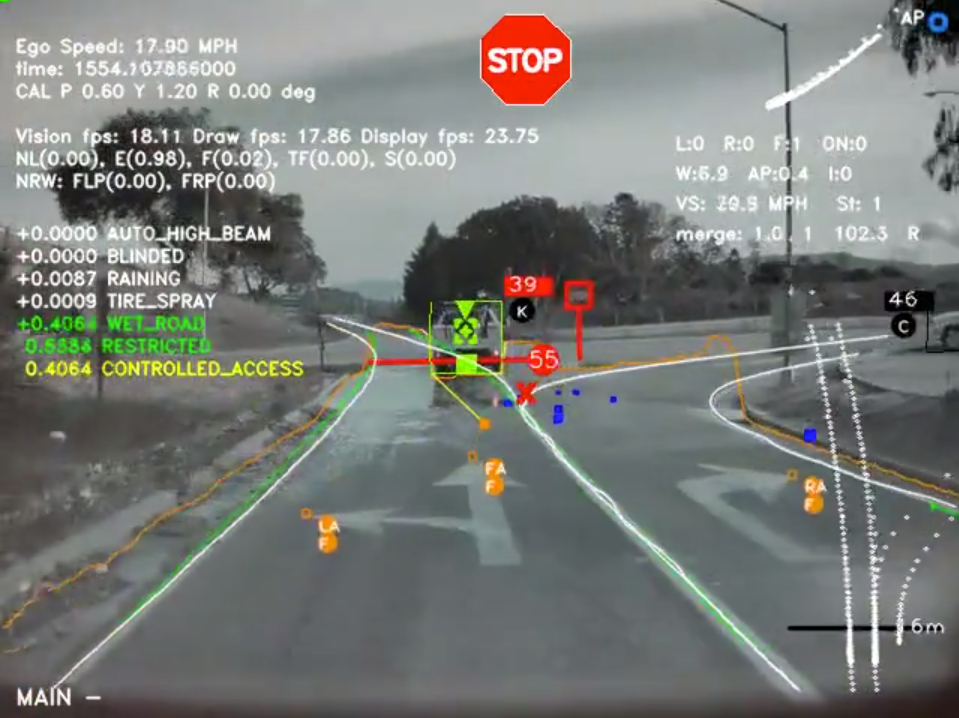
\includegraphics[width=.8\linewidth]{img/teslaautopilotOverlays.png}
      \caption{Fotograma de un video que muestra el comportamiento interno del sistema \textit{autopilot} de los vehículos Tesla}
      \label{fig:teslaautopilotvideorecruit}
    \end{subfigure}%
    \begin{subfigure}[c]{.5\textwidth}
      \centering
      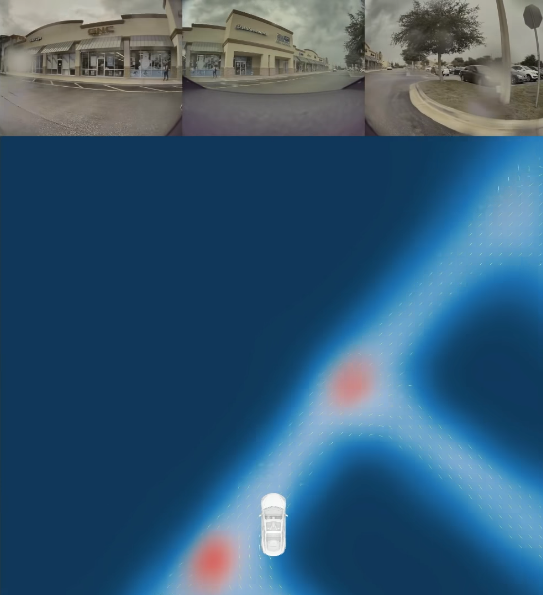
\includegraphics[width=.8\linewidth]{img/teslaTopDown.png}
      \caption{Salida del predictor de calzadas en la vista cenital}
      \label{fig:preditorCalzadasTesla}
    \end{subfigure}
    
    \caption{Ejemplos del funcionamiento interno del sistema Tesla Autopilot}
    \label{fig:ejemploTesla}
\end{figure}

\subsection{Caddillac SuperCruise}

En cuanto al sistema de conducción semiautónoma de Cadillac, SuperCruise, se puede destacar que es un sistema que utiliza mapas de alta resolución generados mediante LIDAR, Radar, GPS y cámaras convencionales para permitir que el vehículo pueda conducir sin la interacción directa del conductor \cite{CaddillacSupercruise}. 

A pesar de que apenas existe información sobre este sistema, ya que tan solo se puede utilizar en varias autopistas de EEUU y Canadá y que la cantidad de personas con acceso a él es mucho menor que a la de los sitemas de sus competidores, en la figura \ref{fig:cadillactobii} se puede observar el dispositivo encargado de controlar la atención del conductor que, ademas de un led indicador, parece tener 6 leds infrarrojos que proyectarán un patrón fácilmente reconocible en la pupila del conductor. Este sistema, parece tener gran similitud con los sistemas de seguimiento ocular para consumidores de la empresa Tobii, uno de los cuales será utilizado en este proyecto.

\begin{figure}[h!]
    \centering
    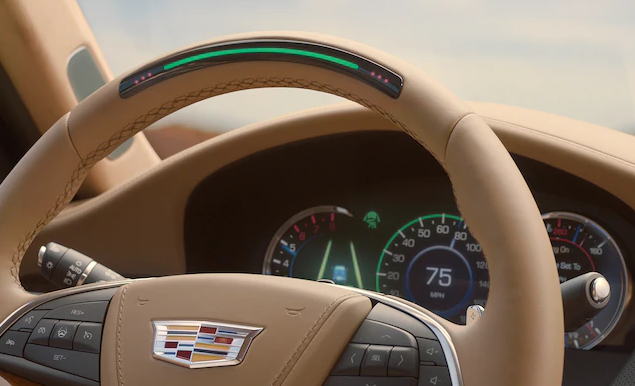
\includegraphics[width=.7\linewidth]{img/cadillacSupercruise.png}
    \caption{Detalle del sistema de control del conductor de Caddillac Supercruise}
    \label{fig:cadillactobii}
\end{figure}

\subsection{OpenPilot}

Openpilot es un sistema de conducción autónoma open-source desarrollado por George Hotz capaz de detectar las líneas de la calzada e interaccionar con el radar de los vehículos compatibles para controlarlo hasta un nivel de autonomía 2. Además también realiza alertas visuales y auditivas ante situaciones anómalas, como por ejemplo la superación del límite de velocidad.
Inicialmente, el sistema se ejecutaba en un teléfono móvil convencional pero posteriormente se ha trasladado a una solución hardware propietaria.

Uno de los puntos interesantes de esta solución es la compatibilidad con más de 85 vehículos de distintas marcas, algo solo posible al tratarse de un proyecto \textit{opensource}.

\begin{figure}[h!]
    \begin{subfigure}[c]{.5\textwidth}
      \centering
      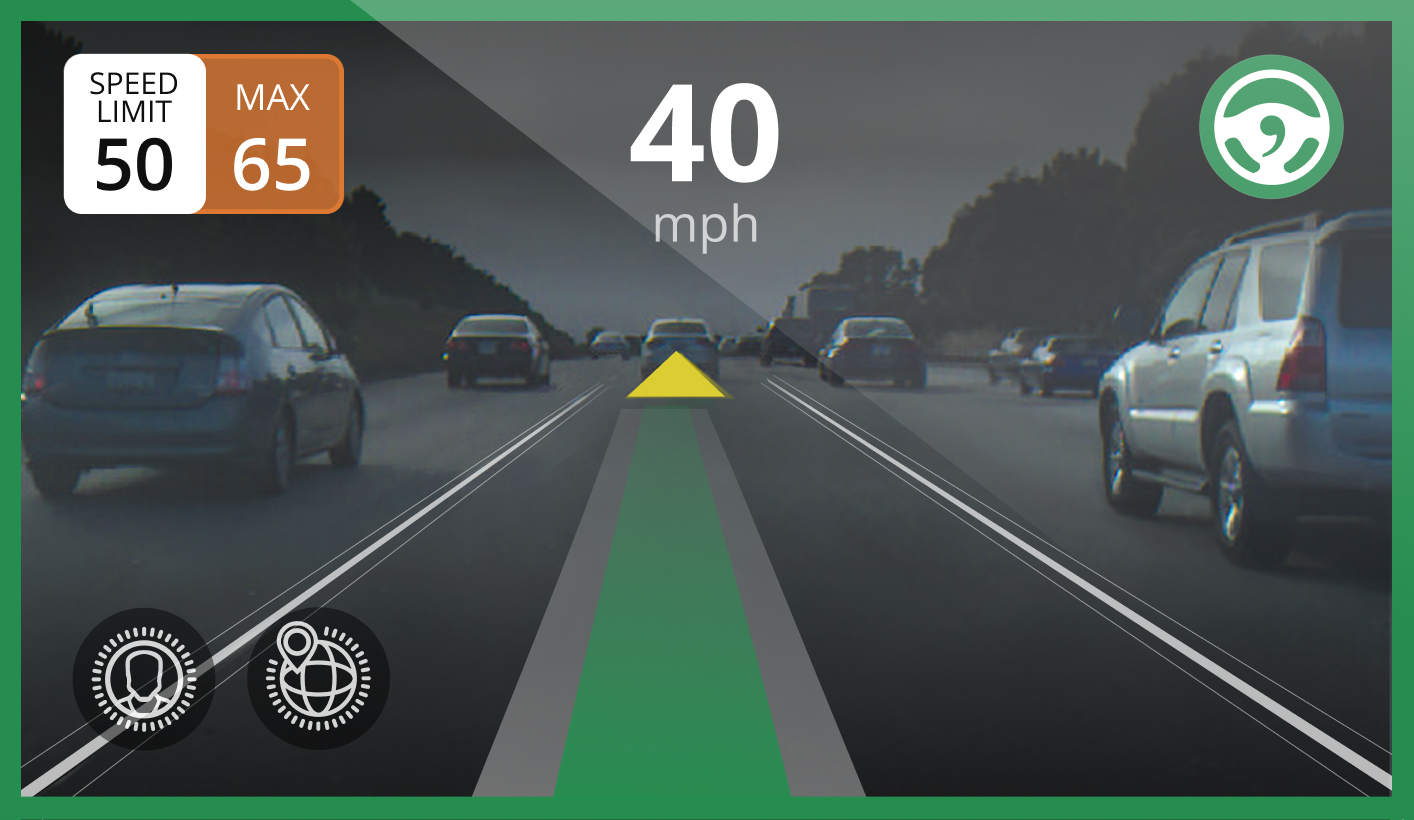
\includegraphics[width=.8\linewidth]{img/Openpilot.jpg}
      \caption{Interfaz gráfica del sistema Openpilot}
      \label{fig:openpilot1}
    \end{subfigure}%
    \begin{subfigure}[c]{.5\textwidth}
      \centering
      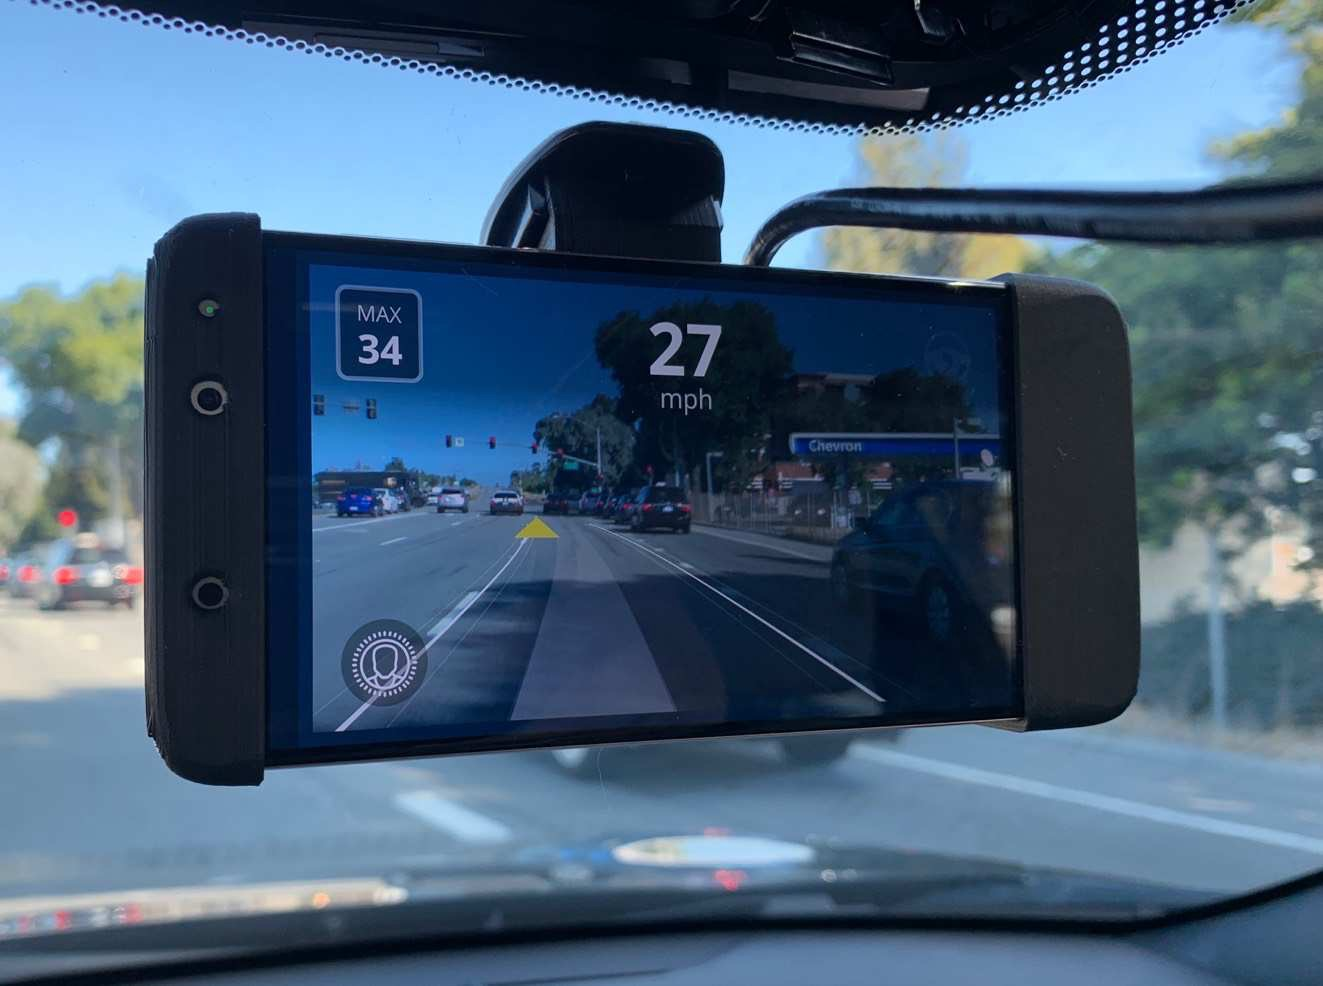
\includegraphics[width=.8\linewidth]{img/openpilot2.jpeg}
      \caption{Ejemplo de uso de Openpilot en un vehículo real}
      \label{fig:openpilot2}
    \end{subfigure}
    
    \caption{Ejemplos del funcionamiento del sistema Openpilot}
    \label{fig:ejemploOpenpilot}
\end{figure}

\section{Elicitación de requisitos}\label{sec:requisitos}

A continuación se indican los requisitos que nuestra aplicación deberá cumplir para considerar una entrega final como satisfactoria.

\begin{itemize}
    \item El sistema deberá recibir la información del vehículo y mostrarla
    \item El sistema deberá ser capaz de reconocer los vehículos a su alrededor
    \item El sistema deberá detectar los cambios de los semáforos
    \item El sistema deberá controlar la atención del conductor
    \item El sistema deberá avisar acústica y visualmente ante situaciones anómalas
\end{itemize}


\section{Análisis de riesgos} \label{sec:analisisriesgos}

Por supuesto, como cualquier otro proyecto es posible que se den algunos problemas. A continuación se describen los posibles riesgos que se pueden dar.

\subsection{Identificación de los posibles riesgos}

\begin{itemize}
    \item Posibles retrasos derivados de las distintas obligaciones del autor\\
        Puesto que la elaboración de este proyecto se realizará en paralelo a la finalización de los estudios del autor y de la entrada al mundo laboral es bastante posible que la priorización de otras tareas no relacionadas con la ejecución del proyecto afecten a los tiempos de desarrollo del mismo.

    \item Pérdida parcial o completa del código fuente\\
        Al trabajar con un proyecto importante siempre es preocupante que debido a problemas de hardware se produzca la pérdida parcial o completa del código fuente.

    \item Imposibilidad del acceso a las herramientas de desarrollo\\
        Otro de los posibles problemas que nos podemos encontrar será la imposibilidad de acceder a las herramientas de desarrollo de nuestro proyecto por causas de fuerza mayor.

    \item Dificultad de implementación\\
        Otro posible riesgo que nos podemos encontrar sería las posibles complicaciones durante la implementación de alguna parte del proyecto. Estas complicaciones podrían aparecer a raíz del desconocimiento de algún tipo de herramienta o librería por parte de los autores.

\end{itemize}

\subsection{Plan de contingencia ante los posibles riesgos}
En el caso de que alguno de los riesgos enunciados anteriormente llegue a materializarse es conveniente conocer las distintas opciones disponibles para minimizar las partes del trabajo que se verían afectadas.

\begin{itemize}
    \item Retrasos en la elaboración del proyecto\\
        La principal solución a los problemas de retrasos consistirá en la reorganización de las tareas y, en el caso de que sea necesario, el retraso de la entrega a las distintas convocatorias disponibles durante el curso escolar.

    \item Pérdida del código fuente\\
        La perdida del código fuente supondría el aplazamiento completo de las tareas y consecuentes retrasos por lo que este es un riesgo que no podemos permitirnos. Afortunadamente, en nuestra industria, la perdida parcial o completa es un riesgo menor gracias a los distintos sistemas que existen para llevar un seguimiento de datos. Para reducir este riesgo y que nunca se llegue a dar, todo el código utilizado en este proyecto se encuentra archivado siguiendo la regla copias de seguridad 321 \cite{backups321}. En concreto, para nuestro proyecto existen al menos 5 copias en 2 medios distintos y con al menos 2 copias \textit{offsite}.

    \item Imposibilidad del acceso a las herramientas de desarrollo\\
        En el caso de que perdamos el acceso a las herramientas de desarrollo de nuestro proyecto o no podamos acceder a ellas por causas de fuerza mayor deberemos modificar la planificación para intentar que el periodo durante el que no tengamos acceso se pueda invertir en otras tareas que no dependan de estas herramientas. Aun así, si este riesgo llegase a materializarse se deberá aceptar el hecho de que los retrasos serán necesarios.
            
    \item Dificultad de implementación\\
        En el caso de que nos encontremos con distintos problemas durante la implementación de alguna parte del proyecto nos veremos obligados a realizar una extensiva investigación para resolver los problemas con los que nos podamos encontrar. Afortunadamente tanto las herramientas como el hardware utilizados parecen estar muy bien documentados y tienen una gran comunidad de personas detrás que nos permitirán, casi con total seguridad, encontrar las respuestas a nuestras preguntas. Si los frutos de la investigación no son suficientes siempre podremos apoyarnos en la ayuda que nuestros tutores nos puedan aportar.

\end{itemize}
	  
	  \chapter{Ejecución del proyecto}\label{capEjecucion}

En este capítulo se podrá encontrar la explicación detallada de las tecnologías consideradas y finalmente utilizadas así como los detalles de la implementación realizada.

\section{Diseño del sistema}\label{sec:diseñosistema}
\subsection{Arquitectura}

\begin{figure}[h!]
    \centering
    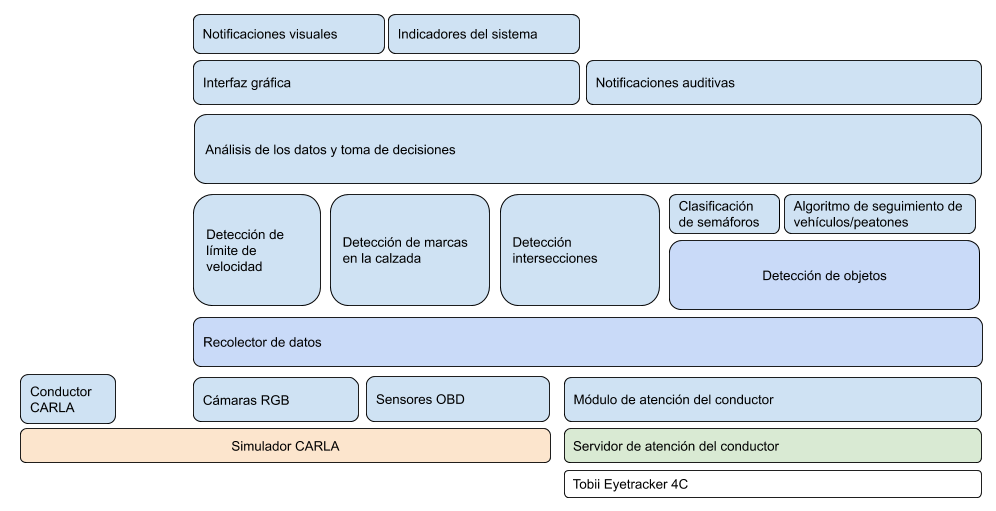
\includegraphics[width=\linewidth]{img/Arquitectura Aplicacion.png}
    \caption{Arquitectura de la aplicación}
    \label{fig:arquitecturaApp}
\end{figure}


La idea principal de la aplicación consiste en la recolección de los datos aportados por el simulador CARLA, en el cual controlamos un vehículo mediante el Conductor CARLA, y el servidor de atención del conductor, que utiliza el sensor Tobii Eyetracker 4C, para posteriormente ser analizados por los distintos módulos de detección y, una vez tengamos conocimiento sobre el estado del vehículo, poder tomar las decisiones y alertar al conductor en el caso de que se crea necesario.


A continuación se comentan con un poco más de detalle los puntos más importantes de entre los que se pueden observar en la figura \ref{fig:arquitecturaApp}:

\begin{itemize}
    \item \textbf{Simulador y conductor CARLA}\\
        El simulador CARLA y la aplicación de conducción nos proporcionarán el mundo y el vehículo sobre el cual se ejecutará nuestro sistema. El usuario tiene control total sobre el vehículo de la misma forma que tendría control sobre un vehículo real.
    \item \textbf{Servidor de atención del conductor}\\
        El servidor de atención del conductor será la pequeña aplicación encargada de controlar la atención del conductor gracias al uso del sensor Tobii Eyetracker 4C
    \item \textbf{Recolector de datos}\\
        El módulo recolector de datos será el encargado de obtener la información del simulador y del servidor de atención del conductor para ponerla a disposición del resto de la aplicación.
    \item \textbf{Módulos de detección}\\
        Una vez obtenidos los datos será necesario analizarlos para obtener conocimiento, este proceso se delega a los distintos módulos que se encargarán de detectar intersecciones, objetos y marcas en la calzada.
    \item \textbf{Análisis de los datos y toma de decisiones}\\
        Cuando se haya obtenido conocimiento acerca de la situación del vehículo será necesario determinar si es necesario emitir alguna notificación. Este módulo será el encargado de realizar esta decisión
    \item \textbf{Interfaz gráfica y notificaciones}\\
        Finalmente, la interfaz gráfica proporcionará un lugar donde podrán observarse todas los datos recogidos así como las notificaciones visuales. Por otra parte, el módulo de notificaciones auditivas permitirá la reproducción de sonidos que alerten al conductor.
\end{itemize}


\clearpage
%-----------------------------------------%
%          Tecnologias consideradas       %
%-----------------------------------------%
\section{Tecnologías consideradas y empleadas} \label{sec:tecnologiasempleadas}
Para la elaboración de este trabajo hemos investigado el uso de distintos dispositivos para obtener información acerca del exterior e interior del vehículo. La mayoría de los dispositivos no han sido utilizados finalmente puesto que se decidió adaptar nuestra aplicación para que funcionase sobre un simulador. Aun así, creemos que es importante aportar información sobre estos dispositivos pues, tal y como se hablará en el capítulo \ref{capTrabajoFuturo}, es posible que en el futuro se utilicen en el caso de que se desee adaptar la aplicación para su uso en un vehículo real.
A continuación se explicarán detalladamente cada uno de estos dispositivos.

\subsection{Tecnologías hardware}
\subsubsection{NVIDIA Jetson AGX Xavier}

\begin{figure}[h!]
    \begin{subfigure}[c]{.5\textwidth}
        \centering
        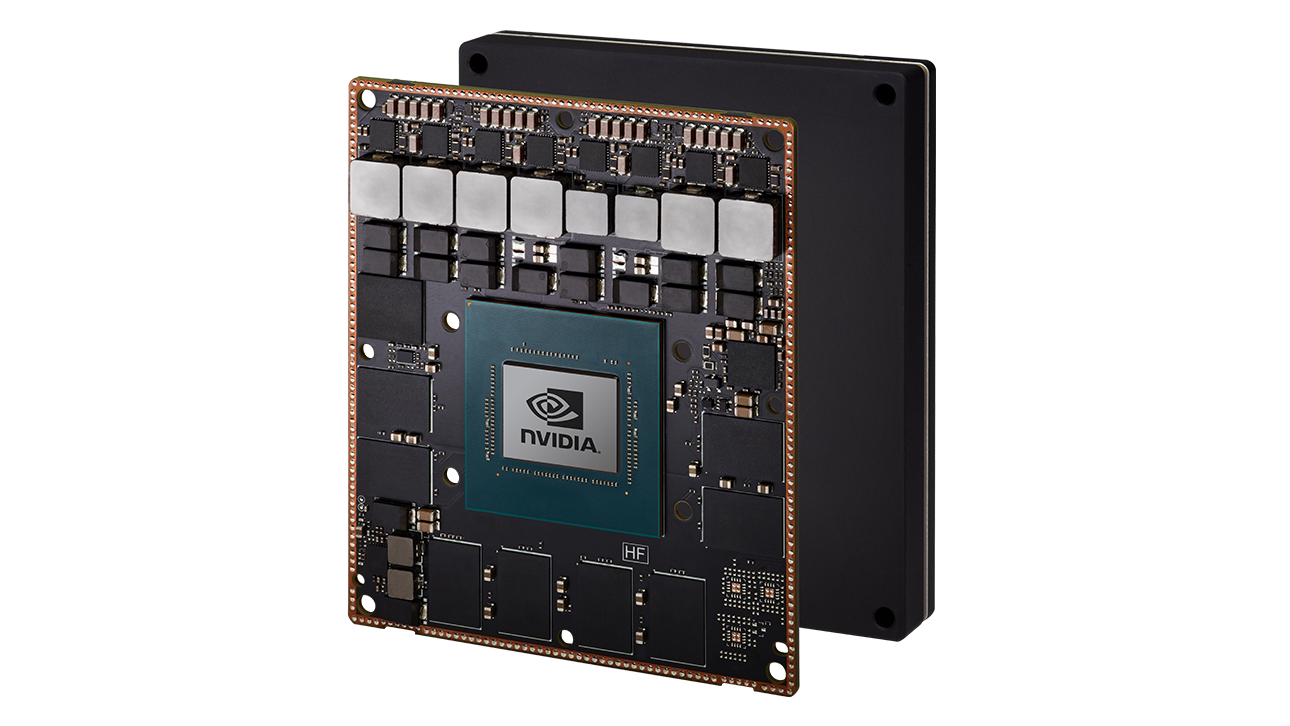
\includegraphics[width=\linewidth]{img/JetsonXavier2.png}
    \end{subfigure}%
    \begin{subfigure}[c]{.5\textwidth}
      \centering
      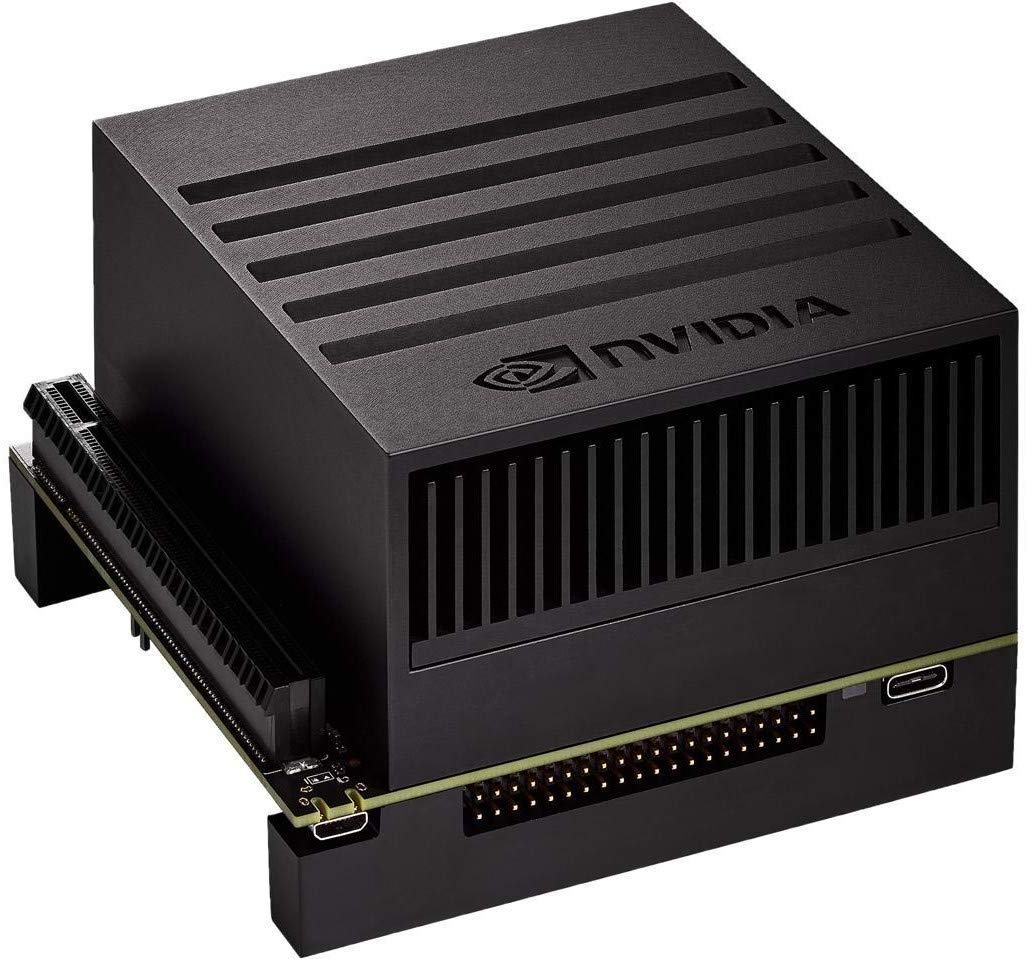
\includegraphics[width=.8\linewidth]{img/jetsonAGX.jpg}
    \end{subfigure}

    \caption{Placa de desarrollo NVIDIA Jetson AGX Xavier y dispositivo con refrigeración integrada}
    \label{fig:jetson}
\end{figure}

La NVIDIA Jetson AGX Xavier se trata de la placa de desarrollo por excelencia para aplicaciones de inteligencia artificial \textit{on the edge} de la compañía NVIDIA.
Está basada en un procesador ARM de 8 núcleos, posee una GPU Volta con 512 \textit{Tensor cores} optimizados para cálculos de inteligencia artificial y 16GB de RAM. NVIDIA asegura que el dispositivo es capaz de alcanzar una potencia computacional de aproximadamente 32 TeraOPS con un consumo máximo de 30W, lo que la hace la opción ideal para la utilización en nuestro proyecto ya que nos permitirá realizar los cálculos necesarios así como las inferencias de los distintos modelos de inteligencia artificial sin que nos tengamos que preocupar por falta de potencia.

En este proyecto utilizaremos la versión con la \textit{carrier board}, que tal y como se puede ver en la figura \ref{fig:jetson} ya tiene incorporado el sistema de refrigeración. 

Uno de los puntos importantes a destacar es que la GPU incluida en este SoC cuenta con 512 \textit{tensorcores}, los cuales son núcleos optimizados para el cálculo de la aritmética utilizada durante la inferencia de los modelos de inteligencia artificial. Gracias a estos núcleos y a la optimización del modelo con la librería TensorRT obtendremos una gran mejora de rendimiento durante la inferencia de los distintos modelos que vamos a crear.

En cuanto a sistema operativo, el dispositivo ejecuta Ubuntu 18.04 sobre la versión 4.9 del kernel de Linux. En este aspecto se puede considerar que la NVIDIA Jetson AGX se trata de un PC normal siendo los únicos puntos a destacar la arquitectura de esta, que es ARM64, y las restricciones de energía.


\subsubsection{Sensores RGBD}

\begin{figure}[h!]
    \begin{subfigure}[c]{.5\textwidth}
        \centering
        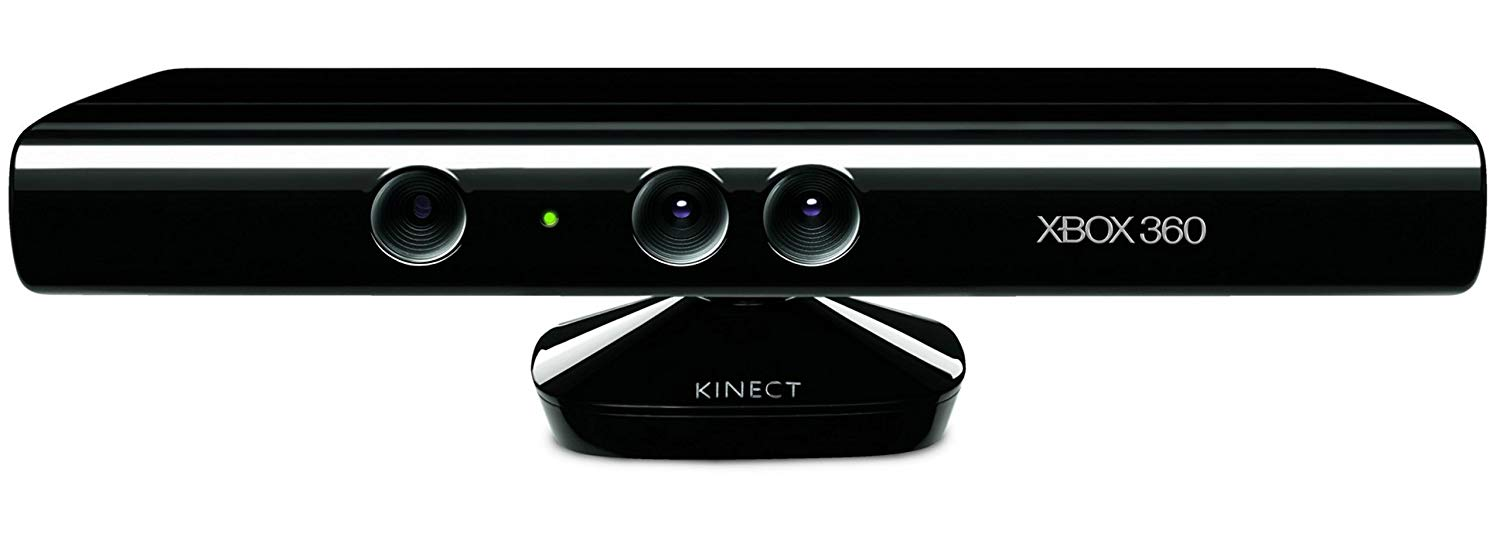
\includegraphics[width=0.9\textwidth]{img/xboxkinect.jpg}
        \caption{Microsoft Xbox 360 Kinect}
    \end{subfigure}%
    \begin{subfigure}[c]{.5\textwidth}
        \centering
        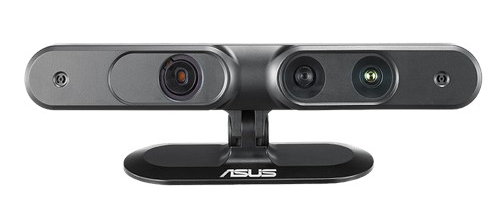
\includegraphics[width=0.9\textwidth]{img/xtionprolive.jpeg}
        \caption{ASUS Xtion Pro Live} 
    \end{subfigure}
    \caption{Aspecto exterior de los dispositivos RGBD}
    \label{fig:dispositivosRGBD}
\end{figure}


Inicialmente se pensó en la utilización de sensores RGBD para la obtención de los datos del exterior del vehículo.

Los sensores RGBD, además de comportarse como una simple cámara RGB también nos aportan un \textit{stream} de datos que nos indica la distancia de cada píxel de la imagen al sensor, generalmente en milímetros.

Estos sensores funcionan de la siguiente forma:

\begin{enumerate}
    \item Una cámara RGB recoge la información de la luz visible de la escena.
    \item Un emisor infrarrojo inunda la estancia en la que se encuentre el sensor con una nube de puntos
    \item Una cámara infrarroja recoge una imagen en el espectro del infrarrojo cercano en la que se pueden diferenciar claramente los puntos del emisor.
    \item Internamente se calcula un \textit{depthmap} del entorno de acuerdo con la calibración de fábrica del dispositivo.
\end{enumerate}

Sin embargo, uno de los problemas de estos sensores es que dependen de la nube de puntos emitida para poder calcular correctamente la distancia de los objetos y para aplicaciones en el exterior, como era nuestro caso antes del cambio al simulador, la nube de puntos se veía completamente eclipsada por la luz solar. 
En la figura \ref{fig:comparativaDephmapRGB} se puede observar un ejemplo de los datos que recibimos desde el dispositivo en una escena exterior.
Finalmente se decidió contra la utilización de este tipo de cámaras puesto que aunque es posible utilizarlas como cámaras RGB normales el tamaño de estas es mucho mayor que el de cualquier cámara RGB, lo que dificulta la instalación de estos sensores en un vehículo real.

\begin{figure}[h!]
    \begin{subfigure}[c]{.5\textwidth}
      \centering
      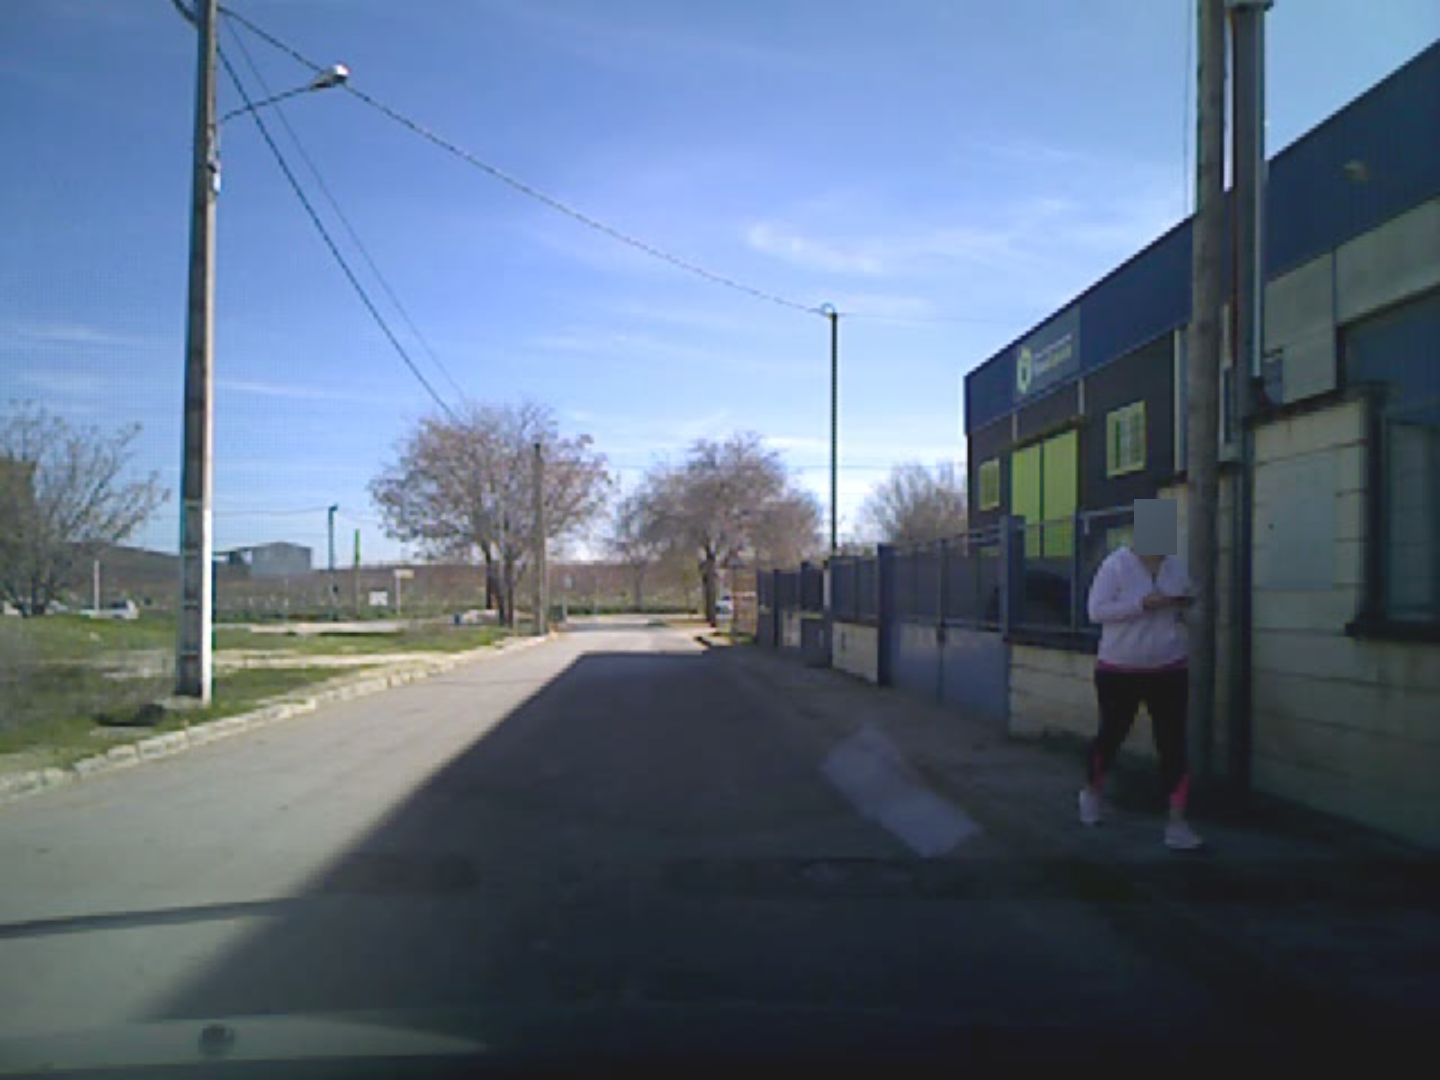
\includegraphics[width=.8\linewidth]{img/comparativaDephRGB/rgb.png}
      \caption{Imagen RGB del dispositivo}
      \label{fig:sfig1}
    \end{subfigure}%
    \begin{subfigure}[c]{.5\textwidth}
      \centering
      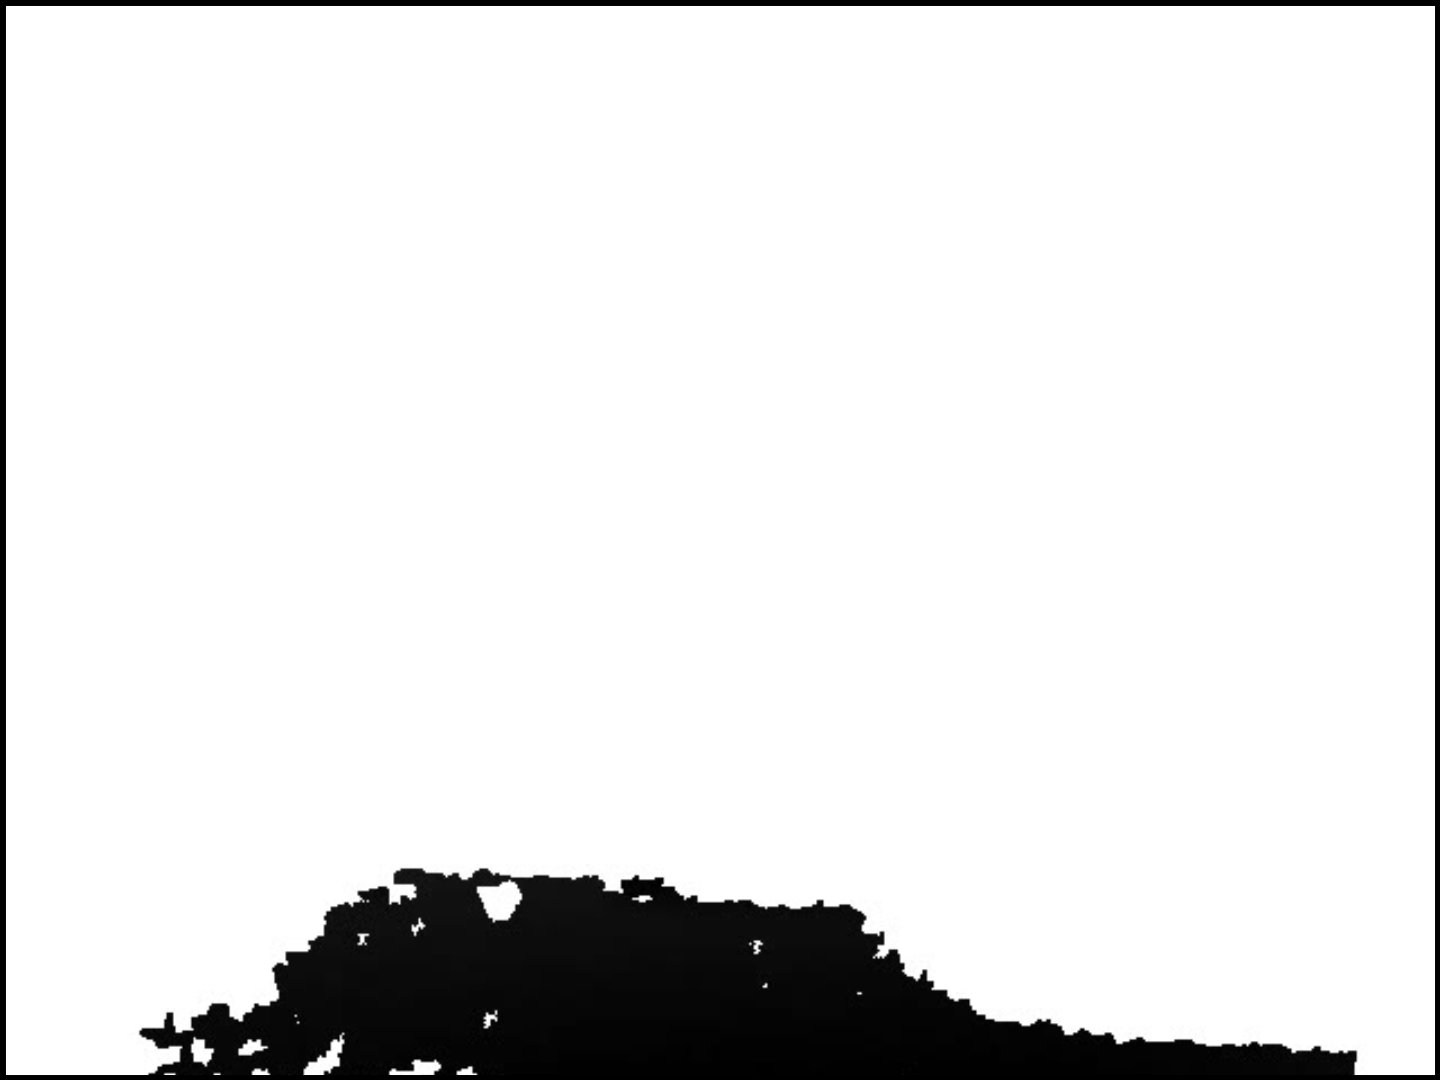
\includegraphics[width=.8\linewidth]{img/comparativaDephRGB/depth.png}
      \caption{\textit{Depthmap} recibido}
      \label{fig:sfig2}
    \end{subfigure}
    
    \caption[Comparativa entre la imagen RGB y el \textit{depthmap} recibido]{Comparativa entre la imagen RGB y el \textit{depthmap} recibido. En este último, el color blanco se corresponde a las regiones sin datos y el negro con regiones demasiado cercanas (reflejos del parabrisas)}
    \label{fig:comparativaDephmapRGB}
\end{figure}

\paragraph{Microsoft XBOX 360 Kinect}\mbox{}\\

El dispositivo Kinect es un periférico de la consola Xbox 360 de Microsoft. Inicialmente desarrollado para competir con otros dispositivos como el mando \textit{PS Move} de Sony y el \textit{Wii Remote} de Nintendo este dispositivo permitía la interacción del usuario en los juegos con todo su cuerpo gracias a la detección del esqueleto del jugador.

En realidad, este periférico no es más que una cámara RGBD que ofrecía los valores de distancia de la imagen capturada a la consola la cual junto con diversos algoritmos realizaba la identificación de la posición del jugador.

Apenas 3 horas después de la salida del dispositivo Héctor Martín ya había creado un driver \textit{open-source} con el que utilizar este dispositivo en un PC \cite{marcan42kinect}. A partir de este punto la comunidad de \textit{makers} comenzó a utilizar este dispositivo en todo tipo de aplicaciones robóticas.


\paragraph{ASUS Xtion Pro Live}\mbox{}\\

El dispositivo ASUS Xtion Pro Live se trata de un dispositivo similar al Kinect que utiliza el mismo tipo de tecnología y del que se pueden obtener los mismos resultados. 

La única diferencia razonable es que este dispositivo es mucho más ligero ya que no incorpora el motor en la base y que funciona únicamente con un cable USB mientras que Kinect necesita una fuente de alimentación externa.

\paragraph{Conclusiones sobre el uso de sensores RGBD}\mbox{}\\
Como ya hemos visto, el uso de este tipo de sensores para la obtención de un \textit{depthmap} no es posible. Sin embargo, también se tuvieron en cuenta otros casos en los que estas cámaras nos podrían haber resultado útiles. 

Una de esas opciones sería la utilización de las dos cámaras al mismo tiempo para obtener una vista estereoscópica de la escena y de esta forma poder calcular la profundidad, una idea especialmente interesante en el caso del dispositivo ASUS Xtion Pro Live, puesto que sus cámaras son simétricas respecto al centro del dispositivo y por su menor peso en comparación con el otro dispositivo a nuestra disposición.
Sin embargo, a pesar de lo que podría parecer a primera vista, ninguno de los dos dispositivos a nuestra disposición son capaces de aportar estos dos streams de datos al mismo tiempo.

Finalmente se decidió contra la utilización de este tipo de cámaras puesto que aunque es posible utilizarlas como cámaras RGB normales el tamaño de estas es mucho mayor que el de cualquier otra cámara RGB, lo que dificulta la instalación de estos sensores en un vehículo real. 


\subsubsection{Sensores RGB}
Una vez visto como los sensores RGBD no eran la mejor opción, pasamos a considerar la opción de cámaras RGB normales.

\paragraph{SONY PlayStation Eye}\mbox{}\\

%\begin{wrapfigure}{r}{0.4\textwidth}
\begin{figure}[h!]
    \centering
    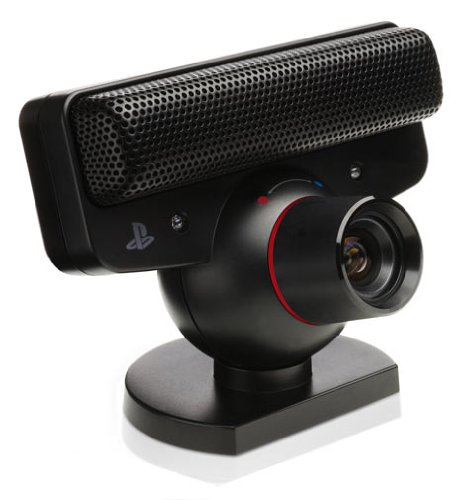
\includegraphics[width=0.25\textwidth]{img/sonyPSeye.jpg}
    \caption{Cámara Sony PlayStation Eye}
\end{figure}
%\end{wrapfigure}

Una de las cámaras consideradas fue la SONY PlayStation Eye. Como su nombre indica, esta cámara es un periférico utilizado por la consola Sony PlayStation 3 para realizar el seguimiento de los mandos con control de movimiento PS Move.

El hecho de que haya sido utilizada por una empresa tan importante como Sony en uno de sus productos principales nos da a entender que esta cámara, a pesar de su reducido tamaño aporta grandes resultados, algo cuyas especificaciones, las cuales se pueden comprobar en la tabla \ref{tab:resFpsPSeye}, parecen corroborar.

Además de ser la calidad de imagen obtenida por la cámara, en la parte superior del dispositivo nos encontramos con una colección de micrófonos que también serán accesibles y que se podrían utilizar para ayudar en el reconocimiento de, por ejemplo, el claxon de otros vehículos o las sirenas de vehículos de emergencias.

\begin{table}[h!]
    \centering
    \begin{tabular}{@{}ll@{}}
    \toprule
    \multicolumn{2}{l}{Especificaciones con parámetros por defecto} \\ \midrule
    Resolución                  & Tasa de refresco                  \\
    640x480                     & 60 FPS                            \\
    320×240                     & 120 FPS                           \\ \midrule
    \multicolumn{2}{l}{Especificaciones con parámetros manuales}    \\ \midrule
    640×480                     & Hasta 75 FPS (con \textit{artefacting})                     \\
    320×240                     & Hasta 187 FPS (con \textit{artefacting})                     \\ \bottomrule
    \end{tabular}
    \caption{Resoluciones y tasas de refresco de la cámara PS Eye}
    \label{tab:resFpsPSeye}
    \end{table}

\paragraph{Aukey PC-LM1}\mbox{}\\

Otra cámara que se consideró utilizar fue la Aukey PC-LM1. Esta cámara, se trata de una \textit{webcam} USB con una resolución de 1080p a una tasa de refresco de 30 FPS. A pesar de que la tasa de refresco sea menor que la que se obtiene con la PS Eye, se pensó que el gran aumento de la resolución nos podría resultar útil para realizar detecciones más precisas.

%\begin{wrapfigure}{r}{0.4\textwidth}
\begin{figure}[h!]
    \centering
    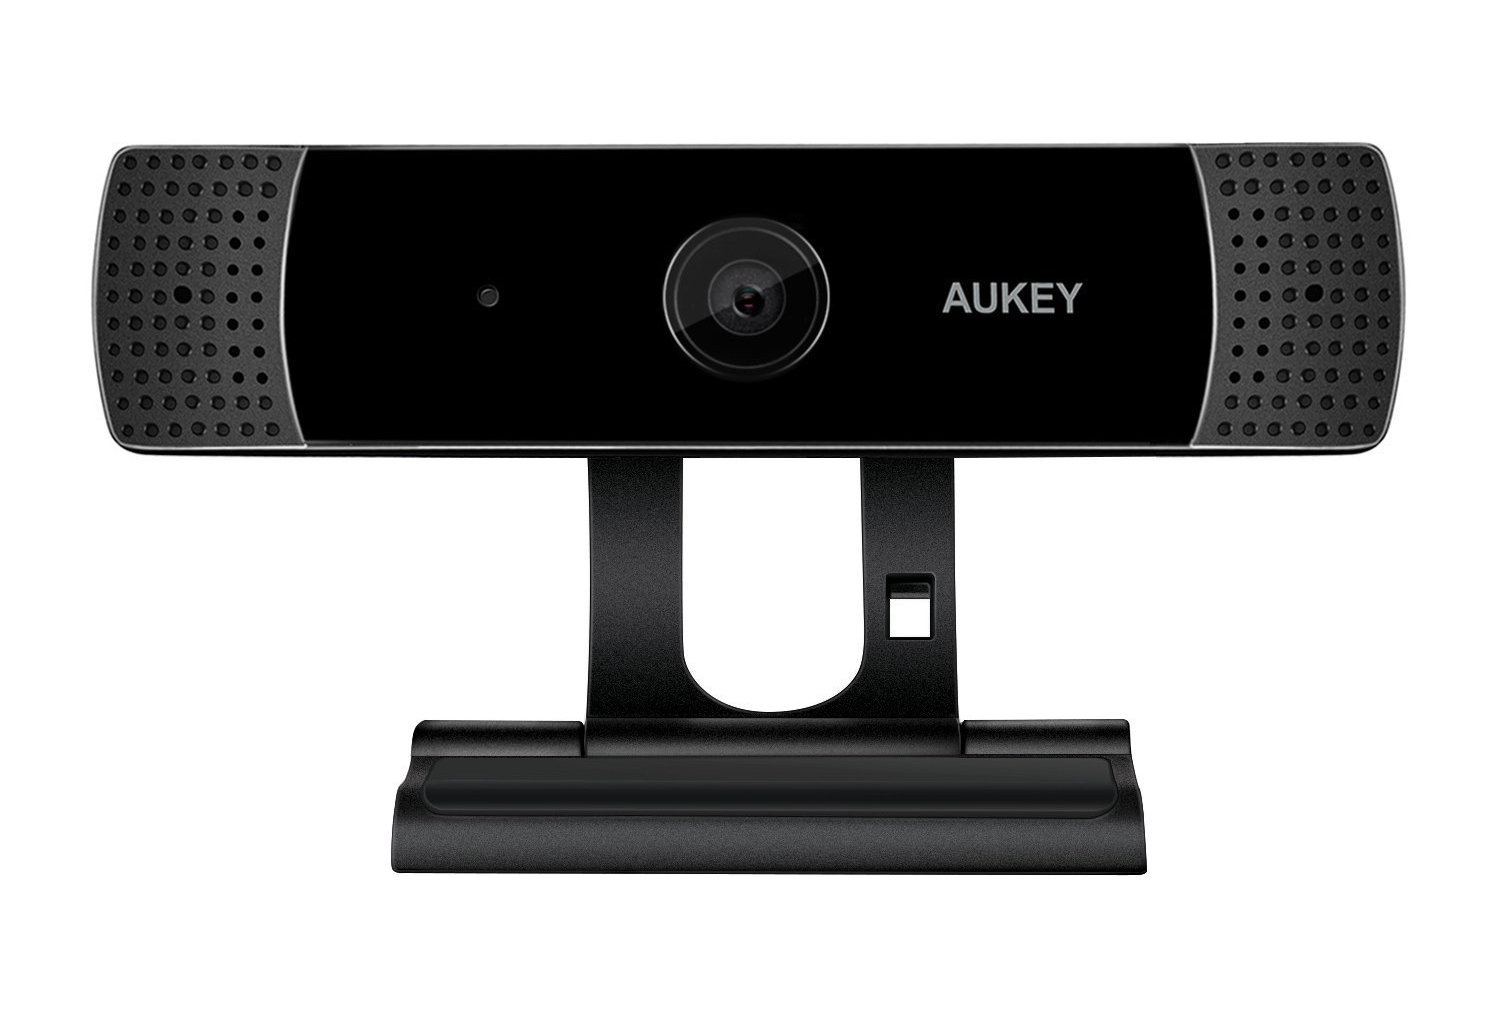
\includegraphics[width=0.35\textwidth]{img/aukeyWebcam.jpg}
    \caption{Webcam Aukey PC-LM1}
\end{figure}
%\end{wrapfigure}


\subsubsection{Conclusiones sobre el uso de sensores RGB y cambio a sensores virtuales}

Tras el cambio del proyecto al simulador CARLA, la utilización de sensores físicos quedó obsoleta puesto que la información del exterior del vehículo se recibiría mediante la API de conexión con el simulador.

\subsubsection{Tobii Eyetracker 4C} \label{sec:tobii}

\begin{figure}[h!]
    \centering
    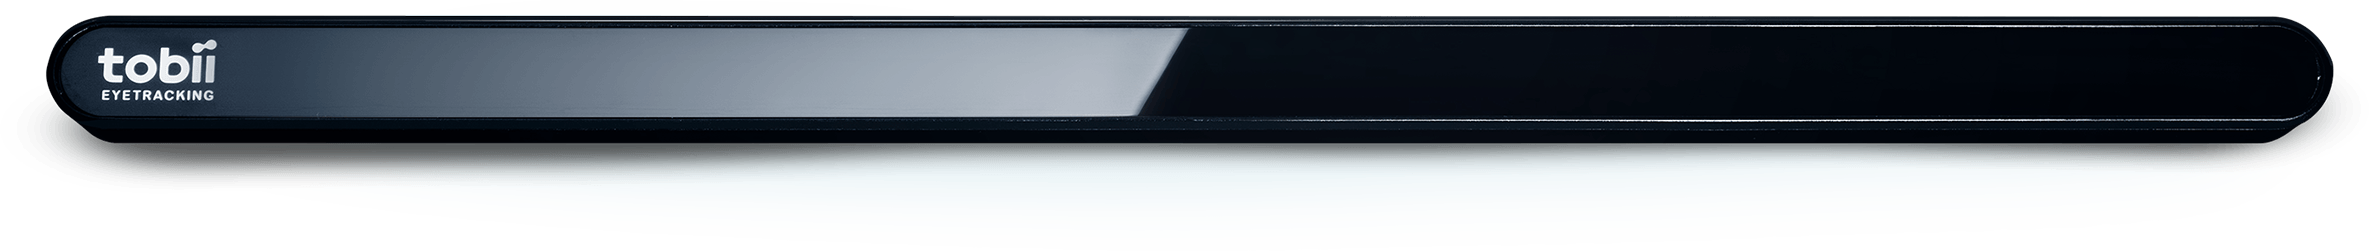
\includegraphics[width=0.6\textwidth]{img/tobii.png}
    \caption{Sensor de seguimiento ocular Tobii Eyetracker 4C}
\end{figure}

Uno de los sensores que si se ha mantenido desde la consideración inicial ha sido el sensor de seguimiento ocular Tobii Eyetracker 4C.
El uso de este sensor nos permite conocer el estado de la visión del conductor y es sin duda uno de los pilares principales de nuestro sistema pues nos permite llevar el control del estado de atención del conductor. 

Existe poca información sobre el funcionamiento del hardware ya que se trata de un producto comercial con precio considerable. Aún así, todo parece apuntar a que varios leds infrarrojos proyectan un patrón fácilmente reconocible en la pupila del usuario el cual es reconocido por las dos cámaras situadas en los extremos del sensor e internamente se calcularán los datos que finalmente se ofrecerán al usuario.

Para acceder a la información obtenida por el sensor Tobii nos ofrece una API con la que podremos obtener distinta información como las coordenadas de la mirada del usuario, la distancia a la mirada y otras más. Sin embargo, como se verá en la sección \ref{sec:sensorAtencion} nuestro dispositivo está bastante limitado al no tratarse de un dispositivo \textit{research}.



\clearpage
\subsection{Tecnologías software}
\subsubsection{Python}

Este lenguaje de programación ha sido seleccionado por la gran facilidad de implementación así como por ser el lenguaje con el que el autor está más familiarizado. Además, dejando de lado la familiaridad del autor con este lenguaje, Python es uno de los lenguaje más utilizados para el prototipado rápido de aplicaciones de \textit{Machine Learning} puesto que existen \textit{bindings} para la mayoría de las librerías y el hecho de que el \textit{overhead} del lenguaje no es excesivamente grande.

\subsubsection{OpenCV}
Para el tratamiento de imágenes se utilizará la librería OpenCV por tratarse de la librería \textit{standard} en tareas de vision por computador con Python. Además, esta librería es relativamente conocida por el autor.


\subsubsection{C\# y WPF}
Para obtener los datos que nos permitan controlar la atención del conductor utilizaremos una aplicación escrita en C\# con el marco de interfaz de usuario Windows Presentation Foundation, que nos permitirá crear una pequeña interfaz gráfica que sea reactiva a la visión del conductor para, de esta forma, saber si el conductor está prestando atención a la calzada o se encuentra distraído.
Como se ha visto en \ref{sec:tobii} utilizaremos las funciones disponibles de la API de Tobii para obtener los datos que se correspondan con la vista del conductor. Concretamente, en nuestro caso haremos reactiva a la vista una ventana y posteriormente utilizaremos las funciones standard de C\# para enviar esta información a la NVIDIA Jetson AGX Xavier.

A pesar del completo desconocimiento del autor de este lenguaje, la gran facilidad de uso así como el gran parecido con Java hacen que programar sea sencillo y que en apenas unas horas se puedan obtener resultados muy buenos.



\subsubsection{Simulador CARLA}\label{sec:simuladorCARLA}

El simulador CARLA \cite{Dosovitskiy17} es un simulador \textit{open source} creado por personal del Toyota Research Institute, Intel Labs y personal del Computer Vision Center de Barcelona.
Está creado con Unreal Engine \cite{unrealengine} y ofrece la ofrece control total sobre los vehículos y el mundo que les rodea por lo que el uso de este simulador está indicado a todas las personas que deseen investigar y desarrollar sistemas de ayuda a la conducción.

\begin{figure}[h!]
    \centering
    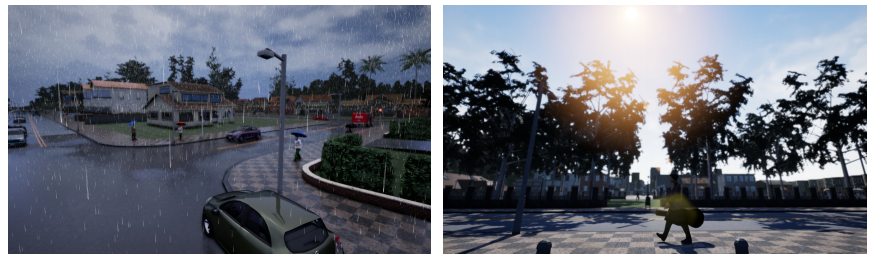
\includegraphics[width=0.85\textwidth]{img/carla1.png}
    \caption{Ejemplos de entornos que se pueden encontrar en el simulador}
\end{figure}

\paragraph{Servidor}\mbox{}\\
CARLA utiliza una arquitectura Cliente-Servidor en la cual el servidor es el encargado de la creación del mundo, el control de los distintos NPCs, ya sean vehículos o peatones, y la renderización de los datos de los sensores.

De entre todos los mapas disponibles en el simulador nos hemos centrado en el mapa Town03 ya que creemos que será posible cumplir nuestros objetivos con el mundo que nos ofrece este mapa.

\paragraph{Vehículos}\mbox{}\\

En la figura \ref{fig:vehiculosCarla} se puede observar una muestra de la diversidad de vehículos disponibles en las primeras versiones del simulador. Desde varias de las últimas versiones del simulador se han incluido diversos cambios que mejoran el comportamiento de los vehículos así como permiten el control de diversos aspectos de los mismos. Uno de los más interesantes y actuales ha sido la inclusión del control de luces.


\begin{figure}[h!]
    \begin{subfigure}[c]{.585\textwidth}
        \centering
        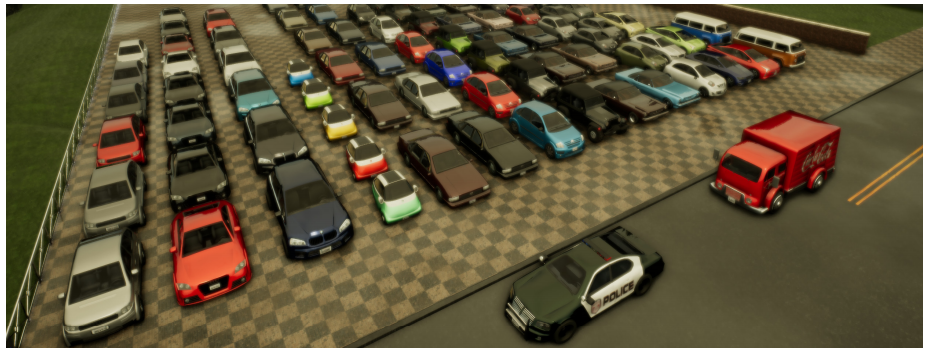
\includegraphics[width=0.9\textwidth]{img/carla3.png}
        \caption{Diversidad de vehículos que se pueden encontrar en el simulador}
        \label{fig:vehiculosCarla}
    \end{subfigure}%
    \begin{subfigure}[c]{.415\textwidth}
        \centering
        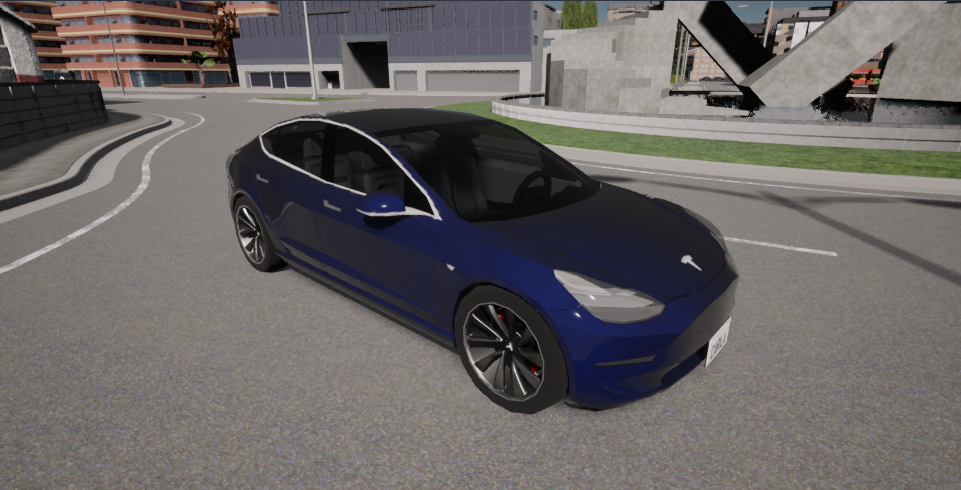
\includegraphics[width=0.9\textwidth]{img/model3.png}
        \caption{Tesla Model 3 en el simulador}
        \label{fig:model3}
    \end{subfigure}
    
    \caption{Diversidad de vehículos en el simulador y vehículos finalmente seleccionado}
    \label{fig:diversidadYmodel3}
\end{figure}




Para nuestro proyecto hemos seleccionado el vehículo Tesla Model 3 ya que se trata de un vehículo que posee amplias cualidades de conducción autónoma en el mundo real y creemos que se trata de una buena base para comenzar nuestro trabajo. Uno de los aspectos que hemos intentado imitar es la posición de las cámaras externas virtuales, las cuales se han colocado aproximadamente en la posición de las cámaras del vehículo real. 

Además al tratarse de un vehículo eléctrico obtendremos una conducción mucho mas suave y no nos tendremos que preocupar por los cambios de marchas, lo que puede ser de ayuda para nuestros algoritmos.


\paragraph{Sensores}\mbox{}\\
En CARLA existen diversos tipos de sensores que podemos añadir a la simulación, en la tabla \ref{tab:sensoresCarlaTabla} se muestran todos los disponibles en la versión 0.99. Dos de los más interesantes y que fueron considerados para la utilización en este proyecto son las cámaras RGB, que por supuesto han sido las utilizadas finalmente, y las cámaras con datos de profundidad, que no se utilizaron finalmente pues trabajar con datos en 3D ampliaría la complejidad de nuestro sistema.

\begin{table}[]
    \centering
    \begin{tabular}{@{}l@{}}
    \toprule
    Sensores disponibles en CARLA      \\ \midrule
    Detector de colisiones             \\
    Sensor de profundidad              \\
    Sensor GNSS                        \\
    Acelerómetro, giroscopio y brújula \\
    Detector de invasión de carril.    \\
    LIDAR                              \\
    LIDAR semántico                    \\
    Detector de obstáculos             \\
    Radar                              \\
    Cámaras RGB                        \\
    Cámara de segmentación semántica   \\
    Cámara DVS                         \\ \bottomrule
    \end{tabular}
    \caption{Sensores disponibles en el simulador CARLA}
    \label{tab:sensoresCarlaTabla}
\end{table}

\begin{figure}[h!]
    \centering
    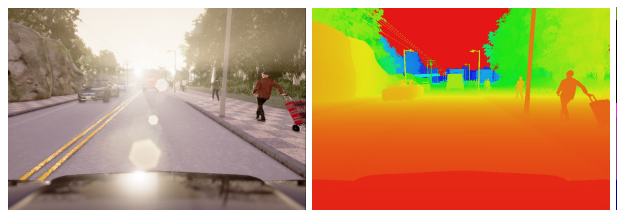
\includegraphics[width=0.8\textwidth]{img/carla2.png}
    \caption[Ejemplos de sensores que se pueden conectar a vehículos]{Ejemplos de sensores que se pueden conectar a vehículos. El primero de ellos es una cámara RGB, el segundo es un sensor de profundidad en escala logarítmica}
\end{figure}


\paragraph{API}\mbox{}\\
Para controlar la simulación y obtener datos se utiliza una API de conexión que nos permite modificar varios parámetros del simulador así como recibir los datos de los sensores que hayamos conectado a algún vehículo.
El único punto a destacar sobre esta API es que no se encuentra disponible para la arquitectura de nuestro sistema y deberá ser compilada para que funcione en la NVIDIA Jetson.



\clearpage
\subsubsection{Interfaz gráfica con Qt5}
\paragraph{Qt Designer}\mbox{}\\

Para el diseño de la interfaz gráfica hemos utilizado el \textit{software} QtDesigner, que nos permite crear interfaces gráficas con la librería Qt5, la cual podremos controlar desde nuestro código python.

El uso de QtDesigner es extremadamente simple y, tal y como se puede observar en la figura \ref{fig:qtdesigner}, recuerda a las herramientas de creación de interfaces de otros \textit{softwares} como Android Studio y Xcode.
Una vez tengamos definida una interfaz necesitaremos transformarla a código python para que la podamos utilizar en nuestra aplicación. Este proceso se realiza mediante el uso de la herramienta \texttt{pyuic} a la cual le aportamos el archivo con la definición de la interfaz y nos devolverá una clase python con la que podremos ejecutar la interfaz.

\begin{figure}[h!]
    \centering
    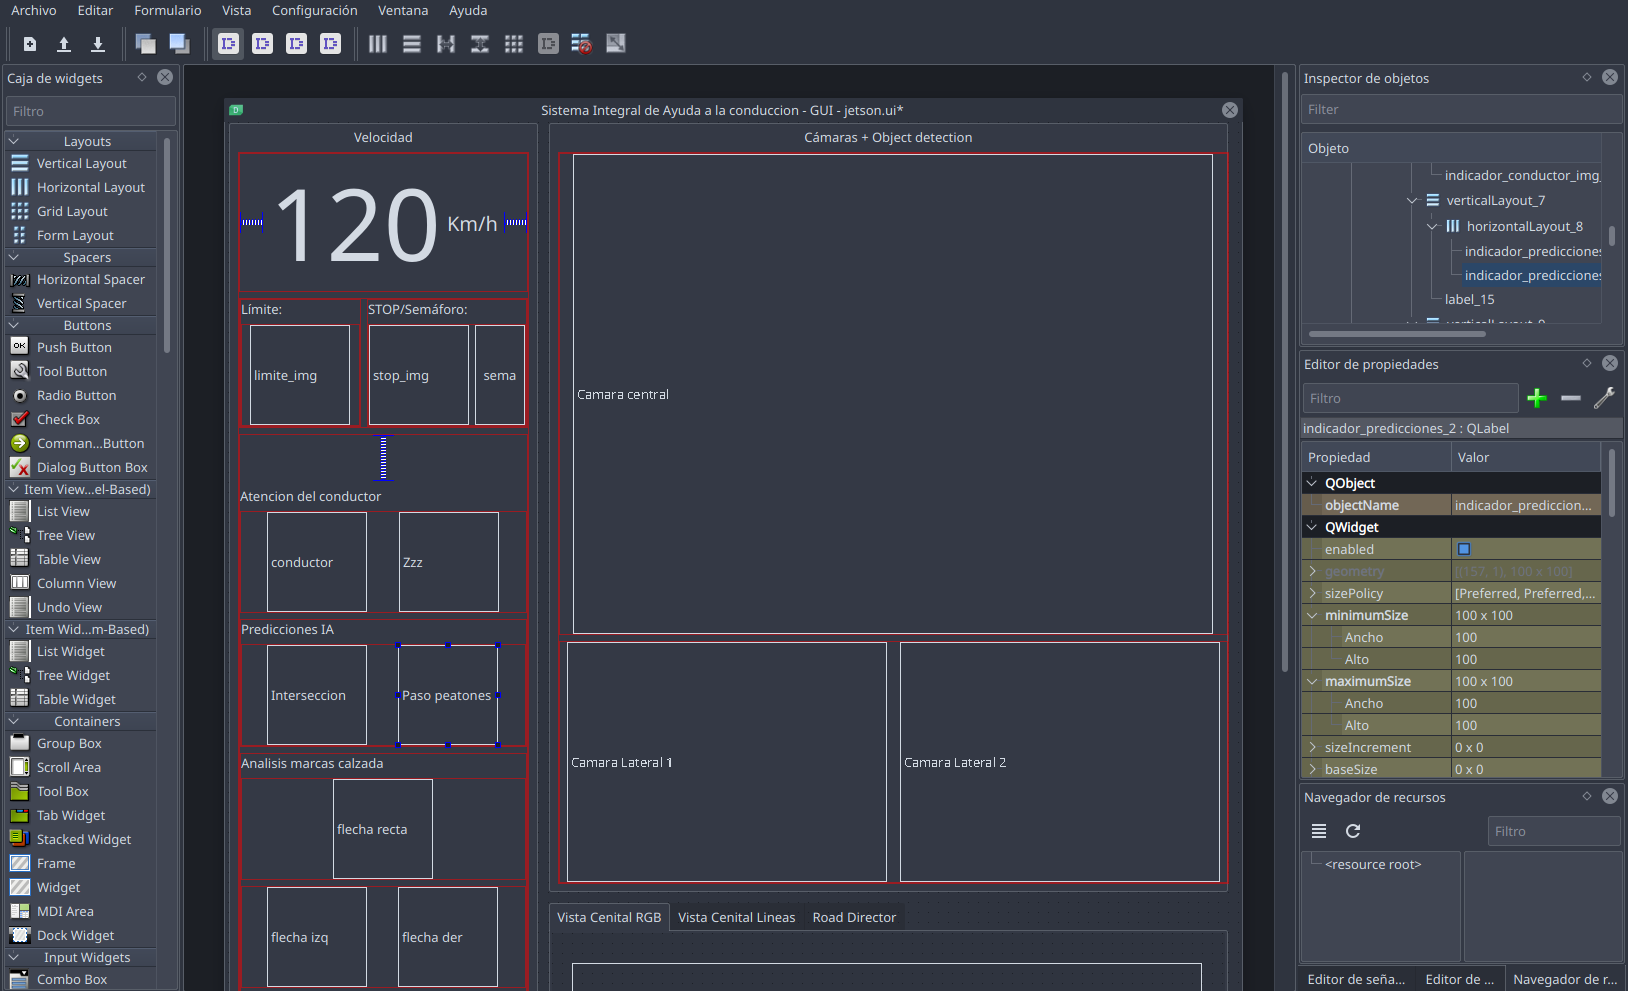
\includegraphics[width=0.8\textwidth]{img/qtdesigner.png}
    \caption{Interfaz del software QtDesigner}
    \label{fig:qtdesigner}
\end{figure}


\clearpage
\subsection{\textit{Datasets} utilizados para el entrenamiento de los modelos} \label{datasets}
A continuación se realiza una pequeña explicación de cada uno de los datasets utilizados para el entrenamiento de los distintos modelos de inteligencia artificial. 

\subsubsection{LISA traffic lights dataset}\mbox{}\\
El dataset LISA \cite{lisaPaper} se trata de un conjunto de imágenes extraídas de unos videos grabados en la parte frontal de un vehículo que han sido anotados para permitir la identificación de distintos tipos de señales de tráfico. Las imágenes han sido grabadas con varios tipos de cámaras por lo que nos encontramos con distintas resoluciones que varían entre 640x480 y 1024x522.


\begin{figure}[h!]
    \begin{subfigure}[c]{.7\textwidth}
      \centering
      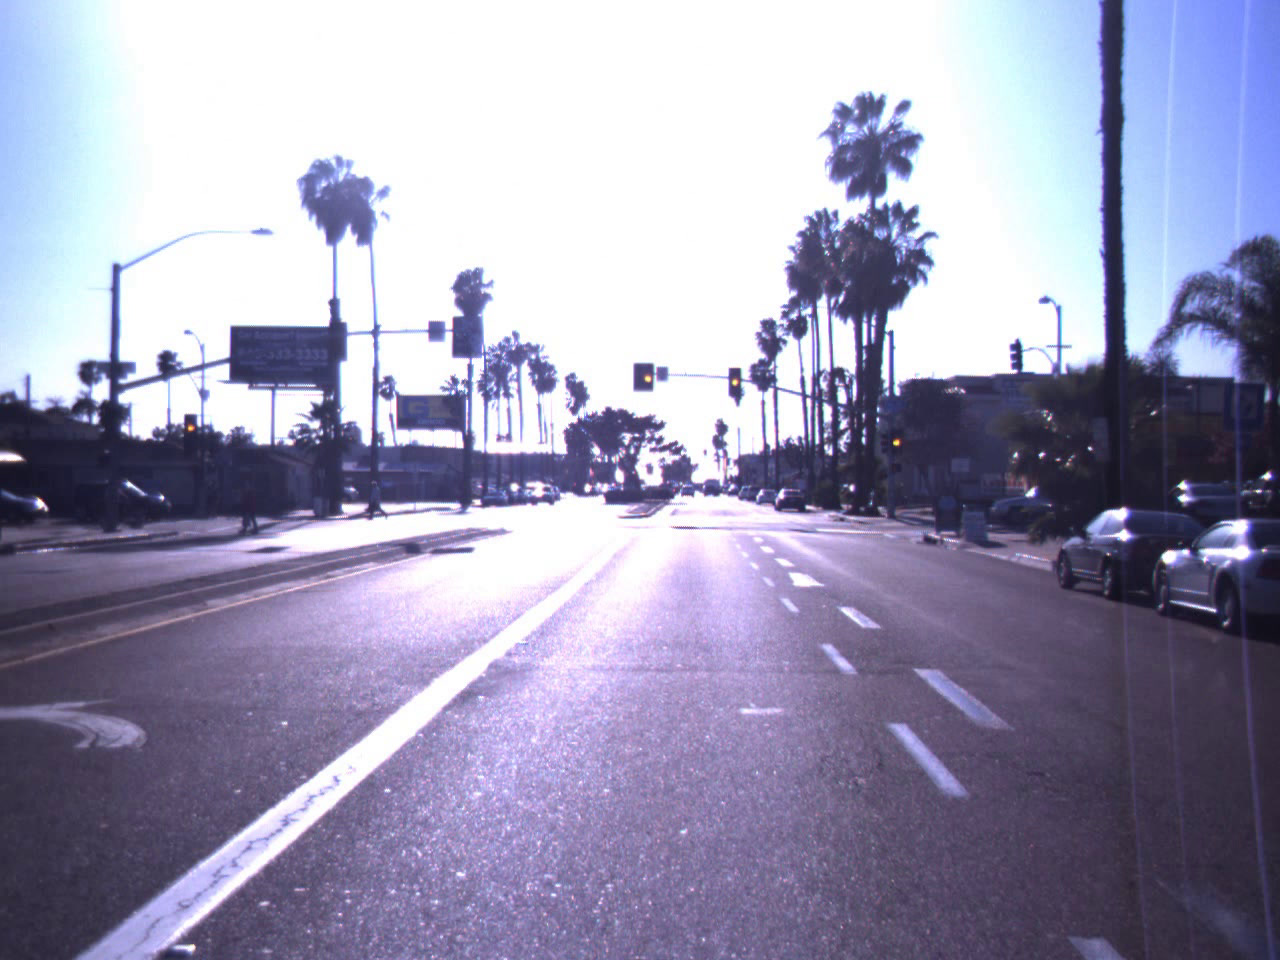
\includegraphics[width=.7\linewidth]{img/ejemploLisa.jpg}
      \caption{Imagen completa}
    \end{subfigure}%
    \begin{subfigure}[c]{.3\textwidth}
      \centering
      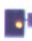
\includegraphics[width=.8\linewidth]{img/recortesemaf.jpg}
      \caption{ Recorte del semáforo }
    \end{subfigure}
    
    \caption{Ejemplo de datos obtenidos con el dataset LISA}
    \label{fig:ejemploLisa}
\end{figure}

El dataset completo contiene 47 tipos de señales y 7855 anotaciones para las 6610 imágenes que nos ofrece.
En nuestro caso hemos reducido este dataset únicamente a la detección de semáforos, por lo que nos hemos quedado con 27518 imágenes para las cuales hemos recortado los semáforos y clasificados en dos grupos, semáforos en verde y semáforos en rojo y ámbar.

\subsubsection{Dataset de intersecciones} \label{sec:datasetIntersecc}\mbox{}\\
El dataset que se ha utilizado para la detección de intersecciones ha sido obtenido por el autor de este trabajo de forma manual.
El dataset consiste en 137 imágenes obtenidas del módulo de análisis de datos, concretamente de la vista cenital de la parte frontal del vehículo.
En la figura \ref{fig:ejemplosintersecc} se pueden observar dos ejemplos de imágenes que contienen este dataset.

\begin{figure}[h!]
    \begin{subfigure}[c]{.5\textwidth}
      \centering
      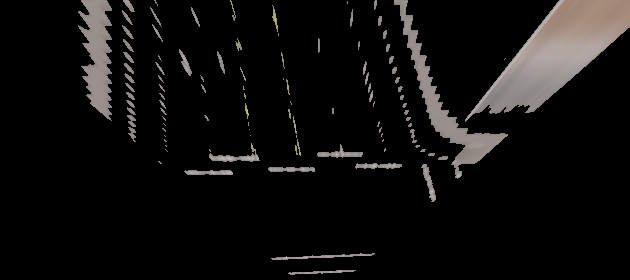
\includegraphics[width=.9\linewidth]{img/ejemploIntersecSi.png}
      \caption{Ejemplo positivo}
      \label{fig:intersSI}
    \end{subfigure}%
    \begin{subfigure}[c]{.5\textwidth}
      \centering
      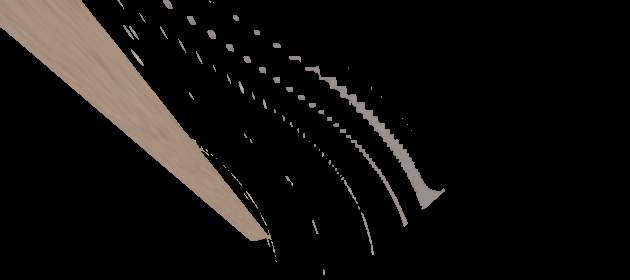
\includegraphics[width=.9\linewidth]{img/ejemploIntersecNO.png}
      \caption{Ejemplo negativo}
      \label{fig:intersNO}
    \end{subfigure}
    
    \caption{Imágenes de ejemplo del dataset de detección de intersecciones}
    \label{fig:ejemplosintersecc}
\end{figure}

\subsubsection{Dataset para \textit{Road Director}}\mbox{}\\ \label{sec:datasetRD}
Al igual que el dataset para la detección de intersecciones, el dataset utilizado para el entrenamiento del modelo \textit{Road Director} se trata de un dataset personal creado con imágenes de la vista cenital del vehículo.
En este caso, el dataset fue creado de forma automática gracias a la funcionalidad ``Autopilot'' del simulador CARLA, la cual permite que el vehículo se mueva por el mapa de forma automática.

Mientras el vehículo se encontrase en movimiento y con una velocidad superior a 3 km/h un pequeño script se encarga de guardar la imágen de la vista cenital inmediatamente delante del vehículo asi como la información de la posición del volante y acelerador.








\clearpage
%-----------------------------------------%
%                DESARROLLO               %
%-----------------------------------------%
\section{Desarrollo} \label{sec:desarrollo}
A continuación se realiza la extensiva explicación de desarrollo realizado para cumplir con los objetivos de este proyecto.

\subsection{Preparando el entorno de desarrollo y despliegue}
\subsubsection{NVIDIA JetPack}
La instalación de NVIDIA JetPack se realiza durante la puesta en marcha del dispositivo NVIDIA Jetson AGX y consiste en la inicialización del dispositivo e instalación de librerías principales.

Para realizar esta inicialización es necesario conectar la Jetson AGX a un ordenador con arquitectura x64 y sistema operativo Ubuntu 18.04 puesto que deberemos instalar el \textit{NVIDIA SDK Manager}, el cual únicamente se encuentra disponible para este sistema. Una vez descargado conectaremos el dispositivo al ordenador y los pondremos en \textit{recovery mode} manteniendo pulsado el botón correspondiente. Una explicación más exhaustiva se podrá encontrar en \cite{manualJetson}.


\paragraph{OpenCV}\mbox{}\\
Tal y como se ha comentado anteriormente, una de las herramientas que utilizaremos en este proyecto será OpenCV y, afortunadamente, al realizar la instalación de JetPack se nos dió la opción de instalar OpenCV al mismo tiempo por lo que una vez se inicialice el dispositivo tendremos acceso inmediato a la librería.

\paragraph{Tensorflow}\mbox{}\\
Al igual que con OpenCV, al realizar la instalación inicial de NVIDIA Jetpack se nos dió la opción de instalar al mismo tiempo Tensorflow.
Al realizar la instalación de esta forma nos aseguramos que Tensorflow se instale correctamente y aproveche sin problemas la GPU del dispositivo puesto que también se instalan automáticamente las distintas dependencias así como CUDA para permitir el uso de la GPU en las inferencias.

La versión de Tensorflow utilizada en este proyecto es la 2.0, concretamente la versión 2.3.0.


\subsubsection{jetson-inference}\label{sec:jetsonInference}

Para utilizar la librería jetson-inference necesitaremos compilarla y por tanto tendremos que obtener el código fuente del repositorio en GitHub\cite{jetsoninferencegithub}.
Tras esto, necesitaremos compilar el repositorio. A modo de resumen, una vez tengamos clonado el repositorio e instaladas las dependencias, estos son los comandos que se deben ejecutar para compilar e instalar la librería:

\begin{lstlisting}[h!, language=bash,caption=Comandos para la compilación de \textit{jetson-inference}]
$ cd jetson-inference
$ mkdir build
$ cd build
$ cmake ../
$ make -j$(nproc)
$ sudo make install
$ sudo ldconfig
\end{lstlisting}

Durante la compilación se nos preguntará qué modelos deseamos instalar junto a la librería. Nuestro sistema es compatible con todos los modelos indicados por la aplicación (a fecha \today) luego es posible instalar todos los modelos disponibles en la sección de \textit{object detection} e ir modificando el código fuente para ver como modifica el comportamiento.

Cabe destacar que es posible que se deseen modificar varios archivos C\+\+ del código fuente de la API \textit{jetson-utils} puesto que si no los modificamos obtendremos una salida constante en la terminal que nos impedirá observar otros tipos de salidas. 
A pesar de que la recomendación sea la de modificar los archivos esta decisión queda a disposición del lector.


\subsubsection{CARLA} \label{sec:preparacionCarla}
Tal y como se ha comentado en la sección \ref{sec:simuladorCARLA} el desarrollo y testeo de nuestro software se ha realizado con el simulador de conducción CARLA \cite{Dosovitskiy17}.

En cuanto a la utilización de CARLA en este proyecto es necesario diferenciar entre dos partes claramente diferenciadas.
Se podrá hacer la distinción entre el servidor CARLA, encargado de la lógica, cálculos y renderizado del mundo y la aplicación de conducción, que creará y ofrecerá el control de un vehículo en el mundo que se está ejecutando en el servidor.

\paragraph{Servidor}\mbox{}\\
La preparación del servidor de CARLA es simple, una vez descargada la \textit{release} deseada procederemos a descomprimir este archivo y a ejecutar el binario \texttt{Carla.sh}. Se recomienda encarecidamente utilizar los parámetros \texttt{--quality-level=Low} y \texttt{--opengl} puesto que mejorará el rendimiento del simulador utilizando unos gráficos más simples y el motor OpenGL el cual se recomienda para los sistemas GNU/Linux por los propios creadores del simulador\cite{carlaOpengl}.

A modo de información, durante la elaboración de este proyecto se ha utilizado la versión 0.9.9 de este simulador, tanto para el servidor como para el cliente y es posible que el funcionamiento entre distintas versiones no sea el correcto ya que pueden existir muchos cambios al tratarse de un proyecto aún en desarrollo.

\paragraph{Conductor}\mbox{}\\
Por otra parte, la aplicación de conducción se trata de un cliente de CARLA que tras conectarse hace aparecer un vehículo en el mundo y nos ofrece el control de este. Gracias a esta aplicación tendremos el control total de un vehículo al que le podemos añadir los sensores deseados para que nuestro software principal pueda entender el estado del vehículo.

\begin{figure}[h!]
    \centering
    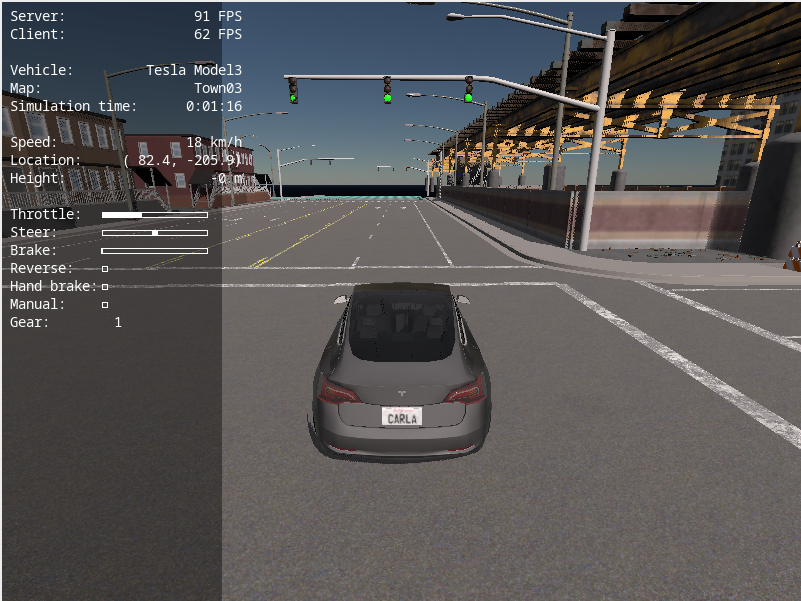
\includegraphics[width=0.8\textwidth]{img/carlaConductor.png}
    \caption{Interfaz de la aplicación de conducción modificada}
    \label{fig:capturaCarlaConduccion}
\end{figure}

La aplicación de conducción se trata de una modificación de los ejemplos de interacción de CARLA, y por lo tanto se encuentra escrita en Python con la ayuda de la librería pygame. En la figura \ref{fig:capturaCarlaConduccion} se puede observar la interfaz de esta aplicación.

Entre las modificaciones realizadas al archivo original se puede destacar la eliminación de los sensores de los que no deseamos recibir datos como por ejemplo el LIDAR y las distintas cámaras de segmentación semántica y de proximidad. Además, también se ha modificado el control del acelerador y freno para que la conducción con teclado sea mucho más suave y realista.


\paragraph{Cliente Python para la NVIDIA Jetson AGX}\mbox{}\\
Para recibir datos en nuestro sistema es necesario conectar nuestra aplicación con el simulador CARLA. Este proceso es bastante sencillo puesto que lo único que debemos hacer es utilizar la API de cliente de CARLA para conectarnos.
Sin embargo, la API de conexión con CARLA no está disponible en los repositorios para la arquitectura de la NVIDIA Jetson AGX por lo tanto tendremos que compilarla manualmente.

Para realizar la compilación de la API de conexión deberemos obtener el código fuente del simulador, el cual se puede obtener en el repositorio oficial en GitHub \cite{repoCARLA}. Una vez hayamos obtenido el código fuente y nos hayamos asegurado de tener todas las dependencias cubiertas procederemos a compilar la API para obtener el archivo \texttt{egg} que posteriormente podremos instalar y de esta forma se nos permitirá importar el módulo \textitt{carla} desde cualquier archivo python.

Una vez se haya instalado la API podremos acceder a los datos generados por el simulador desde nuestro dispositivo tal y como se describe en la sección \ref{sec:datossensores}.


\subsubsection{Entorno Windows 10 para sensor de seguimiento ocular} \label{sec:windows10tobii}
Uno de los principales problemas que supone la utilización del sensor de seguimiento ocular de Tobii es la incompatibilidad de este con nuestro entorno de desarrollo basado en GNU/Linux.
Aunque Tobii asegura que el sensor de seguimiento ocular 4C es compatible con sistemas GNU/Linux, esto es parcialmente cierto puesto que para que sea compatible se deberá utilizar el Pro SDK, un SDK enfocado a los productos \textit{enterprise} de la marca y restringido a tan solo varios de los productos de consumidor.
En nuestro caso, el Tobii 4C se encuentra bajo el grupo de productos de consumidor lo que nos obligaría registrar el dispositivo como un dispositivo \textit{research}, pagando la numerosa cantidad de 2160\euro, para poder utilizarlo con este SDK y de esta forma poder recibir y utilizar información sobre la dirección de la vista del usuario, algo totalmente fuera de nuestras posibilidades.
Sin embargo, bajo sistemas Windows es posible utilizar este dispositivo utilizando el SDK general siempre que no se de un uso que incumpla con la política de uso analítico de Tobii \cite{tobiiAnalyticalUse}.

De esta forma necesitaremos un entorno basado en Windows para poder ejecutar un servidor que nos envíe información, no sobre los datos de la vista del conductor, pues esto incumpliría la política de uso analítico de Tobii, sino la información de interacción del usuario, cuyo uso entraría dentro del uso adecuado de este dispositivo, la interacción del jugador en juegos y aplicaciones de PC.

Para cumplir con este objetivo se ha utilizado un sistema virtualizado basado en Windows Server 2019 al que nos conectamos desde nuestro sistema de desarrollo mediante virt-manager y al que redirigimos el dispositivo de seguimiento ocular. 





\clearpage
\subsection{Obteniendo datos de los sensores} \label{sec:datossensores}
Una vez configurado el entorno de desarrollo podremos pasar a la obtención de los datos desde el simulador.

\subsubsection{Imágenes de las cámaras RGB}

La recolección de imágenes de las cámaras se realiza con el módulo de recolección de datos. Al tratase de las imágenes de las cámaras RGB, recibiremos esta información utilizando las funciones de la clase \texttt{connectCARLAcompleto}.

Para instanciar una cámara RGB deberemos buscar la plantilla y ajustar los parámetros de esta para luego conectarla al vehículo que hemos creado con anterioridad. En el fragmento de código \ref{cod:camaracentral} se muestra la instanciación de la cámara central del vehículo.

\begin{lstlisting}[h!, language=python,caption=Instanciación de la cámara central del vehículo en el simulador,label={cod:camaracentral}]
    camera_bp = blueprint_library.find('sensor.camera.rgb')

    camera_bp.set_attribute('image_size_x', '640')
    camera_bp.set_attribute('image_size_y', '480')
    camera_bp.set_attribute('fov', '56')

    camera_transform_central = carla.Transform(carla.Location(x=0.40, y=0.0, z=1.35))
    camera = world.spawn_actor(camera_bp, camera_transform_central, attach_to=ego_coche)
\end{lstlisting}

La posición de las cámaras puede ser modificada modificando la variable \texttt{camera\_transform\_central} la cual aplicará el \textit{offset} que le indiquemos a la posición que se corresponde con el centro del vehículo. En nuestro caso, las cámaras han sido colocadas aproximadamente en la misma posición que se encuentran las del coche real.

En la figura \ref{fig:imgscams} se puede observar la imágenes de las cámaras que recibimos desde el simulador.
\begin{figure}[h!]
    \centering
    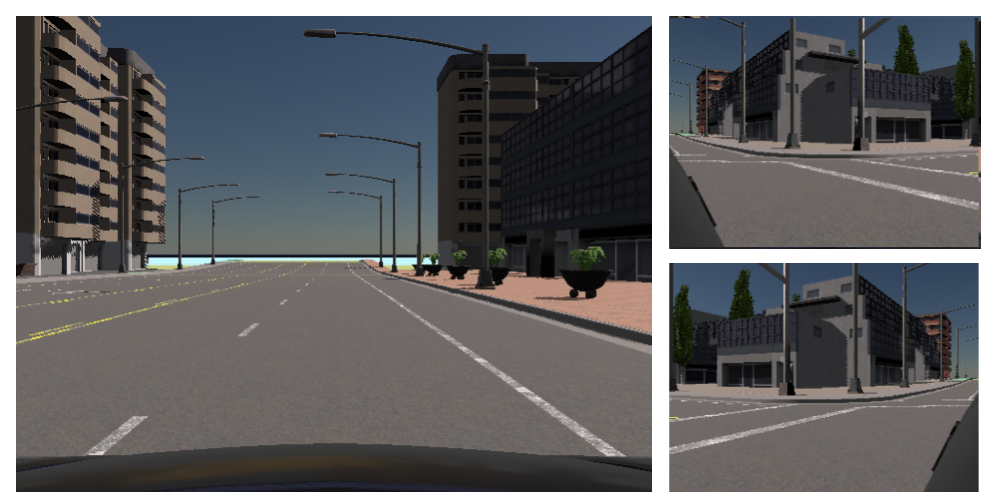
\includegraphics[width=0.8\linewidth]{img/Imagenes camaras.png}
    \caption{Datos de las cámaras recibidos desde el simulador}
    \label{fig:imgscams}    
\end{figure}



\subsubsection{Sensores OBD}
En este apartado hablaremos de otros tipos de sensores que recibimos desde el simulador. Este tipo de sensores se corresponden con los que en un vehículo real podríamos obtener si conseguimos acceso al bus CAN del vehículo.

\paragraph{Velocidad del vehículo}\mbox{}\\
El sensor de velocidad del vehículo, tal y como su nombre indica nos proporcionará la velocidad actual de nuestro vehículo.

Para obtener esta información utilizamos el vector velocidad que podemos obtener desde el simulador y le aplicamos la siguiente fórmula

\begin{equation*}
    3.6* \sqrt{v.x ^2 + v.y ^2 + v.z ^2}
\end{equation*}
donde $v.x$, $v.y$ y $v.z$ son los correspondientes componentes del vector recibido.

Estos datos son actualizados cada 0.03 segundos lo que permite tener gran resolución temporal y reaccionar adecuadamente ante cambios bruscos de velocidad.


\paragraph{Ángulo del volante}\mbox{}\\
Para obtener el ángulo de volante podremos utilizar la función \texttt{get\_control()} del objeto Vehículo de la API de CARLA. Utilizando esta función obtendremos un número entre -0.7 y 0.7 que nos indicará la posición del volante, siendo -0.7 el valor que indica que el volante se encuentra girado completamente a la izquierda y 0.7 que el volante está completamente girado a la derecha.

\paragraph{Límite de velocidad}\mbox{}\\
El siguiente dato que obtendremos será el del límite de velocidad que está afectando al vehículo.
La idea inicial para la detección del límite de velocidad se basaba en la detección de objetos mediante el algoritmo YOLO \cite{yolov3}, sin embargo finalmente 
se decidió utilizar la información que nos devuelve el simulador ya que la implementación no se finalizó a tiempo. 

\subsubsection{Sensor de atención del conductor} \label{sec:sensorAtencion}
Tal y como se ha comentado en la sección \ref{sec:windows10tobii} este sensor se encuentra configurado en una máquina virtual con Windows Server 2019 en la que estamos utilizando un programa que detecta la atención del conductor y envía estos datos a la NVIDIA Jetson AGX Xavier.

Para la creación de este software hemos utilizado la plataforma Windows Presentation Foundation y el lenguaje C\# puesto que la integración con nuestro dispositivo es directa.

La idea principal es utilizar el SDK de Tobii para comprobar si el usuario se encuentra mirando a la ventana de nuestro servidor, que será maximizada, para que de este modo se nos indique si que el conductor se encuentra atento al monitor en el que el simulador está siendo mostrado.

\begin{figure}[h!]
    \centering
    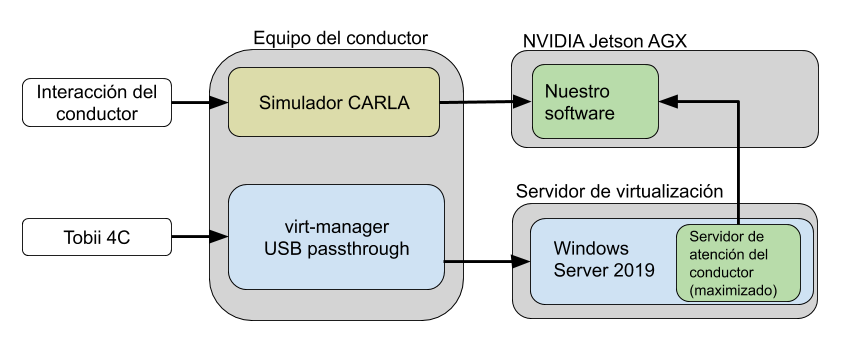
\includegraphics[width=\textwidth]{img/Arquitectura AtencionConductor.png}
    \caption{Arquitectura del sistema de control de atención del conductor}
\end{figure}


\paragraph{Estructura de la aplicación}\mbox{}\\
Una aplicación WPF está generalmente estructurada en dos partes. Archivos \texttt{.xaml} que definen las pantallas y archivos C\# que controlan la lógica de la aplicación.

En nuestro caso hemos definido una vista compuesta por varios elementos, siendo el principal un grid, capaz de reaccionar al evento \texttt{HasGazeChanged} del SDK de Tobii, que nos permitirá saber si el conductor se encuentra mirando a la ventana.

\begin{lstlisting}[h!, language=xml,caption=Grid principal de la aplicación]
    <Grid x:Name="LayoutRoot" 
    tobii:Behaviors.IsGazeAware="True"
    tobii:Behaviors.HasGazeChanged="LayoutRoot_funciontobii">
\end{lstlisting}

También hemos añadido varios cuadros de texto que para que podamos cambiar fácilmente la dirección IP y puerto del cliente al que enviaremos esta información.

\begin{lstlisting}[h!, language=xml,caption=Cuadros de texto para seleccion del servidor y puerto]
    <TextBox x:Name="ip_tbox" HorizontalAlignment="Left" Height="23" Margin="98,35,0,0" TextWrapping="Wrap" Text="10.0.0.6" VerticalAlignment="Top" Width="120" TextChanged="TextBox_TextChanged"/>
    <TextBox x:Name="puerto_tbox" HorizontalAlignment="Left" Height="23" Margin="98,62,0,0" TextWrapping="Wrap" Text="1234" VerticalAlignment="Top" Width="120" TextChanged="TextBox_TextChanged_1"/>
\end{lstlisting}


\paragraph{Obtención del estado del conductor}\mbox{}\\
Para obtener el estado del conductor utilizamos el Grid de la aplicación, el cual, tal y como hemos comentado anteriormente, es reactivo a la visión del usuario gracias a las funciones del SDK de Tobii.

Para tener un control interno de este estado y no solamente modificar el color de nuestra aplicación utilizamos una función que se encarga de modificar una propiedad privada de la clase cuando se produce un cambio en la atención del conductor.



\paragraph{Envío de los datos a nuestra aplicación}\mbox{}\\
Por otra parte, la función encargada de recibir los eventos de cambio de atención también llama a la función encargada de enviar estos datos a nuestro sofware principal.
Este envío de información se produce a través del protocolo UDP. Nuestra NVIDIA Jetson AGX se encontrará escuchando en este mismo puerto a la espera de recibir el paquete enviado por el servidor de atención.
Para la creación del puerto utilizamos las librerías standard de C\# y la única particularidad de esta función es que se están controlando los posibles errores que puedan darse durante el cambio de servidor con un bloque try/catch.



\begin{lstlisting}[float, language=sharpc,caption=Función encargada de enviar los datos a la NVIDIA Jetson AGX,label={cod:servidorUDPwpf}]
public void enviaEstadoConductor()
{
    try
    {
        IPAddress serverAddr = IPAddress.Parse(this.ip);
        IPEndPoint endPoint = new IPEndPoint(serverAddr, this.puerto);

        string estadoConductor = this.conductorPendiente.ToString();

        byte[] buffer = Encoding.ASCII.GetBytes(estadoConductor);
        this.servidor.SendTo(buffer, endPoint);
        Console.WriteLine("Se ha enviado un paquete UDP: " + estadoConductor);
    }
    catch
    {
        IPAddress serverAddr = IPAddress.Parse("127.0.0.1");
        IPEndPoint endPoint = new IPEndPoint(serverAddr, 1234);

        string estadoConductor = this.conductorPendiente.ToString();

        byte[] buffer = Encoding.ASCII.GetByt\begin{lstlisting}[h!, language=sharpc,caption=Función encargada de enviar los datos a la NVIDIA Jetson AGX,label={cod:servidorUDPwpf}]
            es(estadoConductor);
        this.servidor.SendTo(buffer, endPoint);
        Console.WriteLine("Se ha enviado un paquete UDP: " + estadoConductor);
    }
}
\end{lstlisting}




\begin{figure}
    \begin{subfigure}[c]{.5\textwidth}
      \centering
      \includegraphics[width=.95\linewidth]{img/servidorAtenciónRojo.png}
      \caption{Servidor de atención del conductor si el conductor no está atento.}
      \label{fig:atencionCondRojo}
    \end{subfigure}%
    \begin{subfigure}[c]{.5\textwidth}
      \centering
      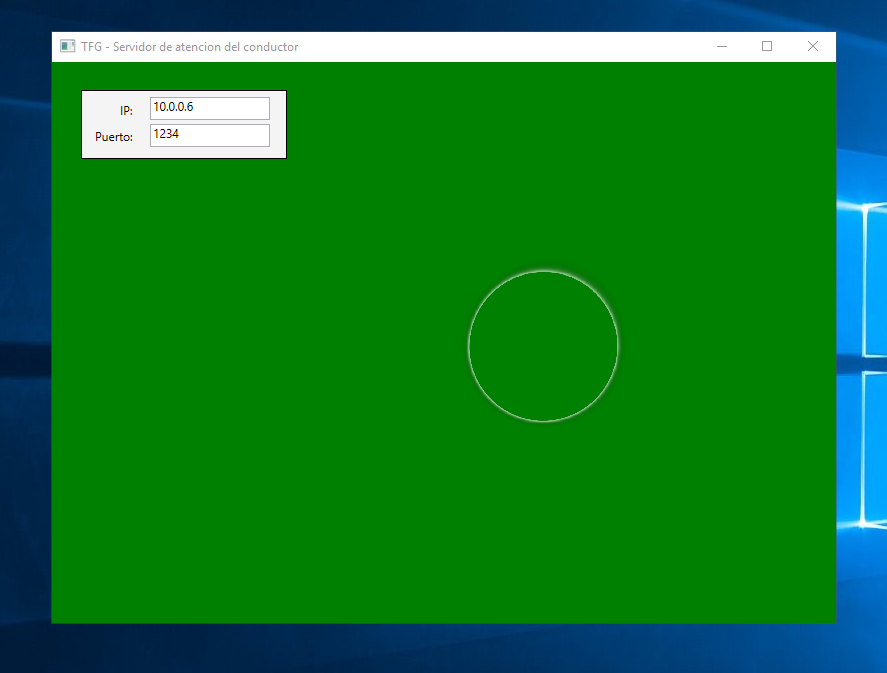
\includegraphics[width=.95\linewidth]{img/servidorAtencionVerde.png}
      \caption{Servidor de atención del conductor cuando este se encuentra atento}
      \label{fig:atencionCondVerde}
    \end{subfigure}
    
    \caption[Servidor de atención del conductor ejecutándose.]{Servidor de atención del conductor ejecutándose. En la figura \ref{fig:atencionCondVerde}, el círculo semitransparente representa la mirada del conductor}
    \label{fig:comparativaDephmapRGB}
\end{figure}


\clearpage
\subsection{Obteniendo conocimiento a partir de los datos adquiridos}

\subsubsection{Detección de intersecciones}
La primera forma de obtener conocimiento será un análisis de la vista cenital del vehículo que nos permita detectar si nos encontramos acercándonos a una intersección.
Para obtener este conocimiento utilizaremos un clasificador binario entrenado sobre el dataset descrito en \ref{sec:datasetIntersecc} en un modelo basado en una simplificación del propuesto por NVIDIA en ``End-to-End Deep Learning for Self-Driving Cars''\cite{nvidiaEndToEnd}. Como se puede observar en la figura \ref{fig:diamIntersecc} únicamente utilizamos 4 capas de funciones Conv2D y 3 capas \textit{fully-connected} frente a las correspondientes 5 y 4 de NVIDIA.
\begin{figure}[h!]
    \centering
    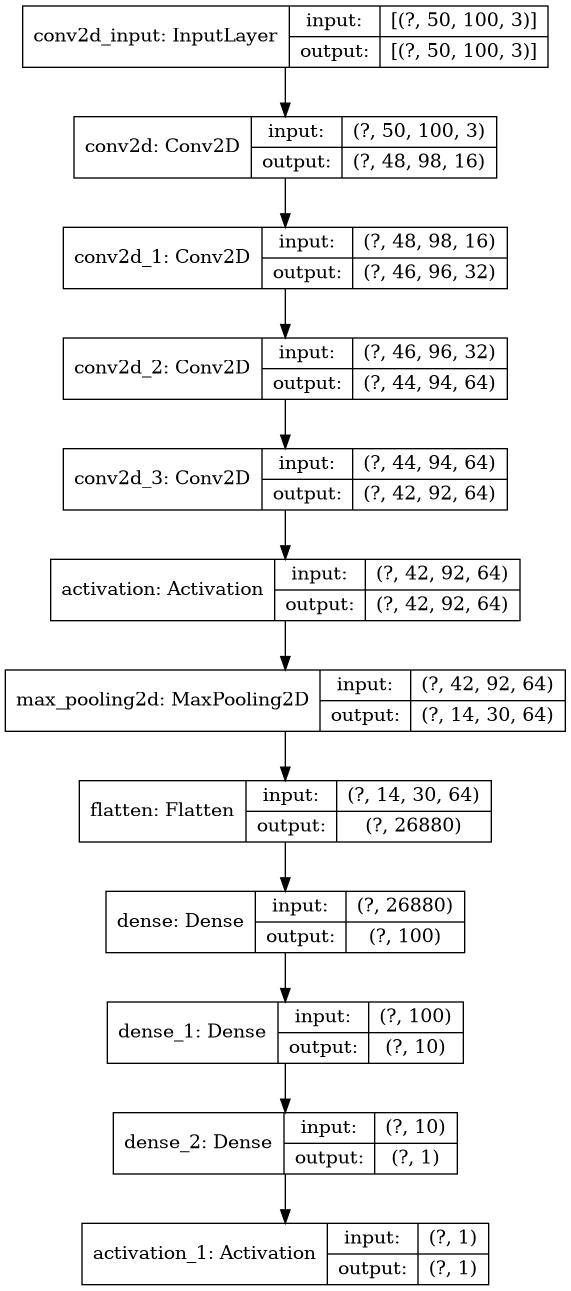
\includegraphics[width=0.6\linewidth]{img/DiagramaIntersecciones.png}
    \caption{Estructura del modelo de detección de intersecciones}
    \label{fig:diamIntersecc}
\end{figure}

Para realizar esta intersección creamos un módulo que se encarga de recibir la imagen cenital y realizar la clasificación. En la figura \ref{fig:imgIntersecc} se puede observar un ejemplo de la imagen que recibe nuestro modelo.
\begin{figure}[h!]
    \centering
    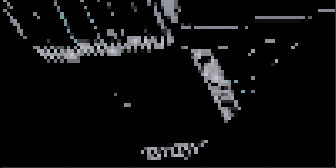
\includegraphics[width=0.6\linewidth]{img/intersecImg.png}
    \caption{Ejemplo de imagen recibida por el detector de intersecciones}
    \label{fig:imgIntersecc}
\end{figure}

El entrenamiento de este modelo se realizó con con los parámetros de la tabla \ref{tab:entrenInteresecc}:
\begin{table}[h!]
    \centering
    \begin{tabular}{@{}ll@{}}
    \toprule
    \multicolumn{2}{l}{Parámetros de entrenamiento del modelo} \\ \midrule
    batch\_size                        & 1024                  \\
    epochs                             & 10                    \\
    validation\_split                  & 0.2                   \\ \bottomrule
    \end{tabular}
    \caption{Parámetros utilizados en el entrenamiento del modelo de detección de intersecciones.}
    \label{tab:entrenInteresecc}
\end{table}



\begin{figure}[h!]
    \begin{subfigure}[c]{.5\textwidth}
      \centering
      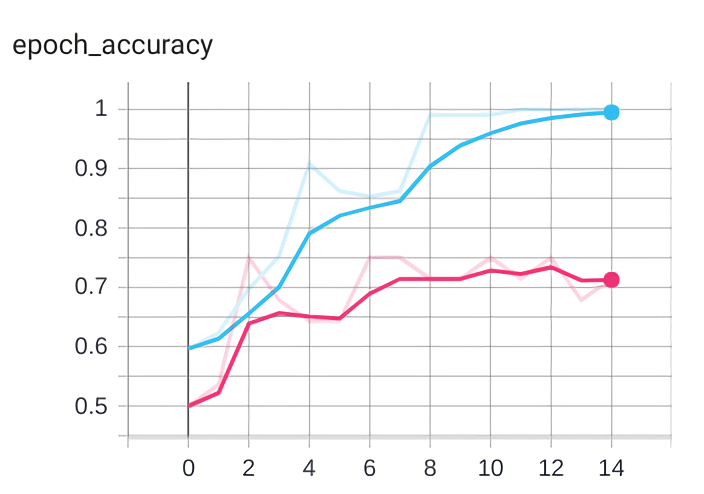
\includegraphics[width=.9\linewidth]{img/interseccionesAcc.png}
      \caption[Precisión del entrenamiento del modelo de intersecciones]{Evolución de la precisión durante el entrenamiento}
      \label{fig:interseccionesAcc}
    \end{subfigure}%
    \begin{subfigure}[c]{.5\textwidth}
      \centering
      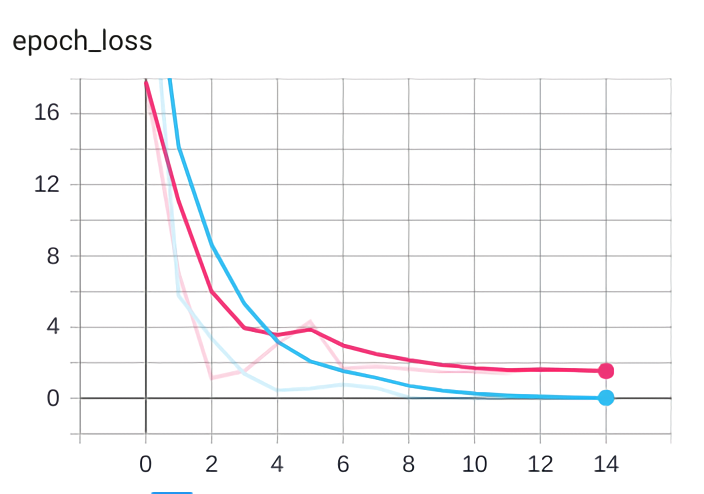
\includegraphics[width=.9\linewidth]{img/interseccionesLoss.png}
      \caption[\textit{Loss} del entrenamiento del modelo de intersecciones]{Evolución de la función \textit{loss} durante el entrenamiento}
      \label{fig:interseccionesLoss}
    \end{subfigure}
    
    \caption[Métricas obtenidas durante el entrenamiento del detector de intersecciones]{Métricas obtenidas durante el entrenamiento de la red convolucional. Las líneas azul y rosa indican la precisión y \textit{loss} sobre el conjunto de entrenamiento y validación respectivamente.}
    \label{fig:graficasInters}
\end{figure}

Una vez finalizado el entrenamiento podremos comprobar los datos que se han obtenido durante este, los cuales se encuentran disponibles en la figura \ref{fig:graficasInters}, y veremos que los valores de precisión sobre el subset de validación no son muy buenos. Aun así, tras un testeo extensivo el resultado de este modelo es bastante satisfactorio puesto que consigue distinguir claramente si nos encontramos acercándonos a una intersección correctamente. Los bajos valores de la precisión se podrán explicar por el pequeño número de ejemplos que nuestro dataset posee.


Una vez testeado el modelo se procede a la optimización de este, la cual convertirá el modelo en un modelo de TensorRT y permitirá la ejecución de este en la GPU de nuestra NVIDIA Jetson AGX Xavier. La optimización del modelo se realiza con la ayuda del script que se puede observar en el fragmento de código \ref{cod:TRT}.



\begin{lstlisting}[float, language=python,caption=Script utilizado para convertir un SavedModel de tensorflow a un modelo optimizado de TensorRT,label={cod:TRT}]
import tensorflow as tf
import sys
from tensorflow.python.compiler.tensorrt import trt_convert as trt

path = sys.argv[1]

conversion_params = trt.DEFAULT_TRT_CONVERSION_PARAMS
conversion_params = conversion_params._replace(precision_mode="FP16")
conversion_params = conversion_params._replace(maximum_cached_engiens=100)

converter = trt.TrtGraphConverterV2(input_saved_model_dir=path, conversion_params=conversion_params)
converter.convert()
converter.save(f'{path}_optimizadoTRT_FP16')    
\end{lstlisting}

\clearpage
\newpage

\subsubsection{Detección de objetos}

Para cumplir uno de los objetivos principales del proyecto deberemos encontrar distintos tipos de objetos en la imagen de las cámaras, siendo los principales los vehículos y peatones.

Para ello, aprovechando la arquitectura modular de nuestra aplicación hemos creado un módulo que nos permita realizar la detección de objetos de una forma sencilla, únicamente deberemos pasarle la imagen de la cámara deseada y nos devolverá una lista con los objetos que ha detectado.

En cuanto a la detección de objetos en si utilizamos la librería \textit{jetson-inference} que nos permitirá aplicar diversos modelos de inteligencia artificial de una forma muy sencilla y con gran rendimiento en los sistemas NVIDIA Jetson.

El modelo que hemos utilizado con esta librería ha sido \textit{ssd-mobilenet-v2} que por supuesto se trata de la segunda versión del famoso modelo SSD de mobilenet entrenado en las 80 clases del \textit{dataset} COCO \cite{lin2014microsoft}.

\begin{table}[h!]
    \centering
    \begin{tabular}{@{}lll@{}}
    \toprule
    \multicolumn{3}{c}{Objetos del dataset COCO}  \\ \midrule
    person        & tie            & chair        \\
    bicycle       & suitcase       & couch        \\
    car           & frisbee        & potted plant \\
    motorcycle    & skis           & bed          \\
    airplane      & snowboard      & mirror       \\
    bus           & sports ball    & dining table \\
    train         & kite           & window       \\
    truck         & baseball bat   & desk         \\
    boat          & baseball glove & toilet       \\
    traffic light & skateboard     & door         \\
    fire hydrant  & surfboard      & tv           \\
    street sign   & tennis racket  & laptop       \\
    stop sign     & bottle         & mouse        \\
    parking meter & plate          & remote       \\
    bench         & wine glass     & keyboard     \\
    bird          & cup            & cell phone   \\
    cat           & fork           & microwave    \\
    dog           & knife          & oven         \\
    horse         & spoon          & toaster      \\
    sheep         & bowl           & sink         \\
    cow           & banana         & refrigerator \\
    elephant      & apple          & blender      \\
    bear          & sandwich       & book         \\
    zebra         & orange         & clock        \\
    giraffe       & broccoli       & vase         \\
    hat           & carrot         & scissors     \\
    backpack      & hot dog        & teddy bear   \\
    umbrella      & pizza          & hair drier   \\
    shoe          & donut          & toothbrush   \\
    eye glasses   & cake           & hair brush   \\
    handbag       &                &              \\ \bottomrule
    \end{tabular}
    \caption{Objetos del dataset COCO}
    \label{tab:CocoObj}
\end{table}

Para nuestro uso, las clases más importantes serán aquellas que se correspondan con vehículos, personas y señales de tráfico. Para estas clases además, hemos creado una clase distinta en python para poder añadirle distintos parámetros como por ejemplo, en el caso del vehículo, si nos encontramos acercándonos a él o la posición predecida en los siguientes frames. A modo de ejemplo en el fragmento de código \ref{cod:constVeh} se muestra el constructor de la clase vehículo.
    
\begin{lstlisting}[float, language=python,caption=Constructor de la clase personal de vehículos,label={cod:constVeh}]
def __init__(self, objNvidia, idLoop):
    # Datos NVIDIA
    self.Area = objNvidia.Area
    self.Bottom = objNvidia.Bottom
    self.Center = objNvidia.Center
    self.ClassID = objNvidia.ClassID
    self.Confidence = objNvidia.Confidence
    self.Height = objNvidia.Height
    self.Instance = objNvidia.Instance
    self.Left = objNvidia.Left
    self.Right = objNvidia.Right
    self.Top = objNvidia.Top
    self.Width = objNvidia.Width

    # Datos personales
    self.Centro = centroPersonal(objNvidia)
    self.ID = idLoop
    self.numeroFramesSinDeteccionNueva = 0 # Para controlar frames en los que no se detecte


    # Memorias de las ultimas 8 posiciones
    self.memoriaTop = deque([], 8)
    self.memoriaTop.append(objNvidia.Top)

    self.memoriaBottom = deque([], 8)
    self.memoriaBottom.append(objNvidia.Bottom)

    self.memoriaRight = deque([], 8)
    self.memoriaRight.append(objNvidia.Right)

    self.memoriaLeft = deque([], 8)
    self.memoriaLeft.append(objNvidia.Left)

    # Prediccion -> Inicialmente el mismo 
    self.predictTop = int(objNvidia.Top)
    self.predictBottom = int(objNvidia.Bottom)
    self.predictLeft = int(objNvidia.Left)
    self.predictRight = int(objNvidia.Right)

    self.AcercandoseOalejandose = None
\end{lstlisting}


Para realizar la inferencia llamamos a la función \texttt{deteccionRGBframe640} para las imágenes de la cámara central y \texttt{deteccionRGBframe320} para las laterales puesto que estas tienen la mitad de la resolución.
\begin{lstlisting}[float, language=python,caption=Función encargada de realizar la inferencia con el modelo de detección de objetos, label={cod:inferObj}]
def deteccionRGBframe640(self, frame):
    # Lo convertimos a RGBA
    frame = cv2.cvtColor(frame, cv2.COLOR_RGB2RGBA)

    # Lo pasamos a CUDA para que se pueda usar con la net
    frame = jetson.utils.cudaFromNumpy(frame)

    detections = self.net.Detect(frame, 640, 480)

    frame = jetson.utils.cudaToNumpy(frame, 640, 480, 4)
    frame = cv2.cvtColor(frame, cv2.COLOR_RGBA2RGB).astype(np.uint8)

    self.detections = detections
    self.frame = frame
    self.fps = self.net.GetNetworkFPS()

    return self.detections, self.frame, self.fps
\end{lstlisting}
    




\subsubsection{Transformación de perspectiva sobre las imágenes de las cámaras}

Para obtener la vista cenital a partir de la imagen de las cámaras será necesario cambiar la perspectiva de la vista utilizando las funciones de OpenCV para este cometido.

En concreto utilizaremos la función \texttt{warpPerspective} que utilizaremos en conjunción con una matriz de transformación de perspectiva definida a partir de cuatro puntos de nuestra imagen.
En la figura \ref{fig:persWarpDiam} se puede ver el proceso de aplicación de esta función y en el fragmento de código \ref{cod:transcentral} se indica el código necesario para transformar la perspectiva de la camara central.

\begin{figure}[h!]
    \centering
    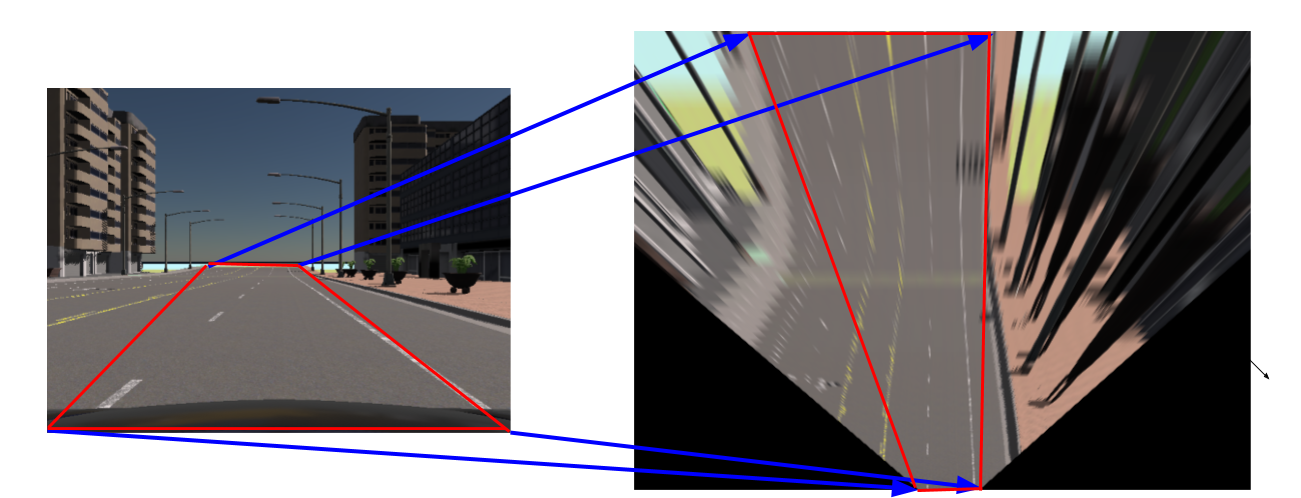
\includegraphics[width=.95\linewidth]{img/PerspectivaWarp.png}
    \caption{Aplicación del cambio de perspectiva}
    \label{fig:persWarpDiam}
\end{figure}

\begin{lstlisting}[float, language=python,caption=Fragmento de código encargado de realizar la transformación de perspectiva de la cámara central, label={cod:transcentral}]
src = np.float32([[300, 250], [350, 250], [0, 480],   [640, 480]])
dst = np.float32([[280, 0],   [370, 0],   [300, 480], [350, 480]])

M = cv2.getPerspectiveTransform(src, dst)

topDown = cv2.warpPerspective(camaraCentral, M, (640, 480))
\end{lstlisting}


\begin{figure}[h!]
    \begin{subfigure}[c]{.33\textwidth}
      \centering
      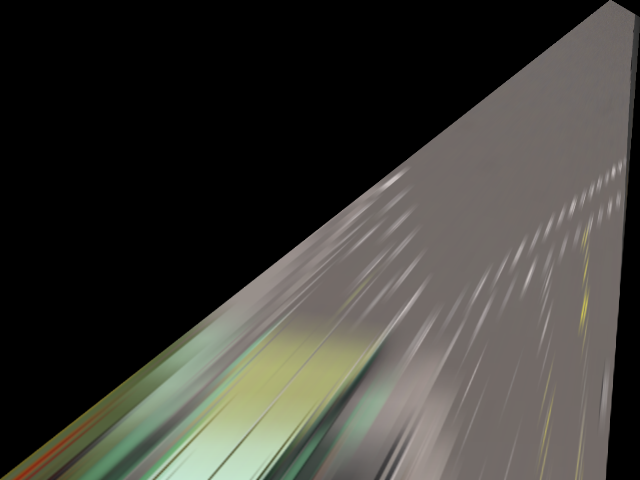
\includegraphics[width=.9\linewidth]{img/warp2.png}
    \end{subfigure}%
    \begin{subfigure}[c]{.33\textwidth}
      \centering
      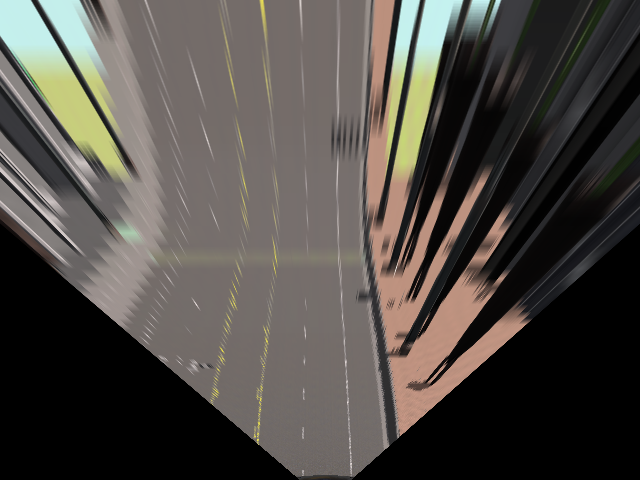
\includegraphics[width=.9\linewidth]{img/warp1.png}
    \end{subfigure}%
    \begin{subfigure}[c]{.33\textwidth}
        \centering
        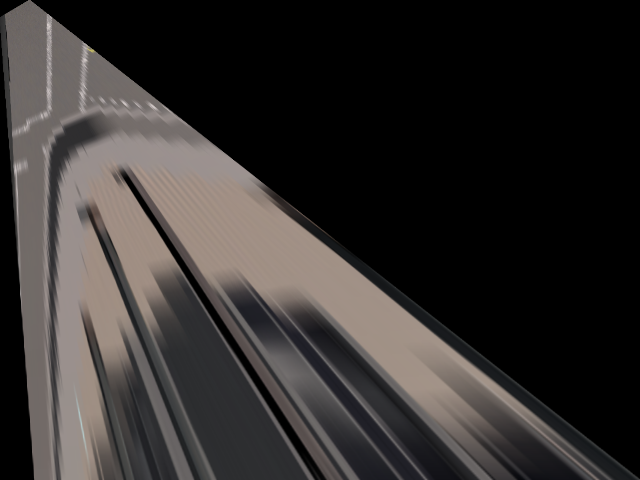
\includegraphics[width=.9\linewidth]{img/warp3.png}
    \end{subfigure}
    
    \caption{Imágenes de las cámaras con el cambio de perspectiva}
    \label{fig:wapimg}
\end{figure}

Una vez obtenidas las imágenes que se pueden observar en la figura \ref{fig:wapimg} procederemos a unirlas para obtener una vista cenital como la que se puede ver en la figura \ref{fig:persWarp}
\begin{figure}[h!]
    \centering
    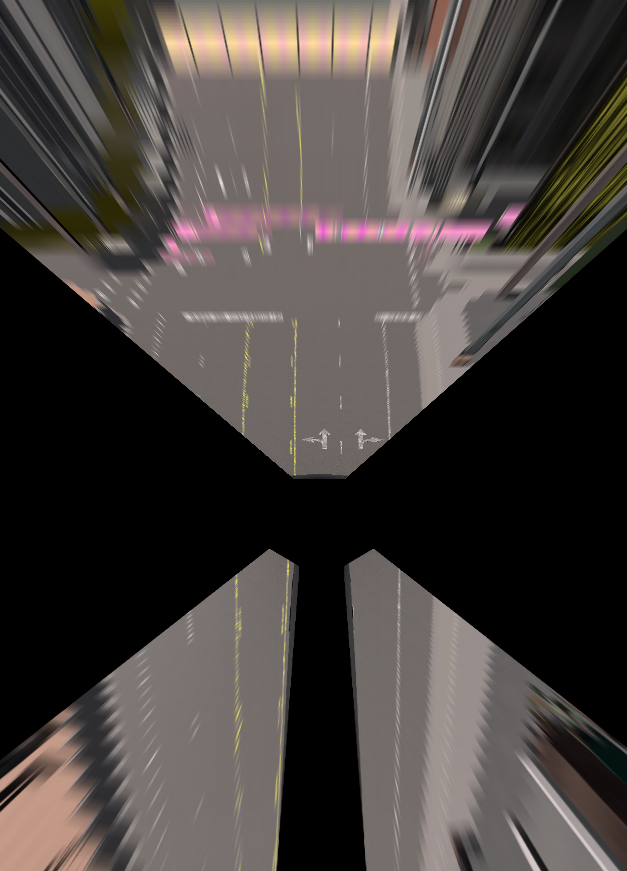
\includegraphics[width=.9\linewidth]{img/persWarpRGB.png}
    \caption{Vista cenital de la zona alrededor del vehículo}
    \label{fig:persWarp}
\end{figure}










\subsubsection{Detección de marcas de la calzada}
Una vez obtenida la vista cenital de la zona alrededor del vehículo podremos intentar detectar las marcas en la calzada.

\paragraph{Filtrado de la imagen para obtener marcas en la calzada}\mbox{}\\
Antes de comenzar con la detección deberemos aislar las marcas en la calzada de toda la imagen.
Para realizar esta separación convertimos la imagen al formato HLS y aplicamos un filtro sobre el canal L. Esto nos separará las marcas de la calzada del resto de la imagen pues estas tienen un valor de L mucho mayor que los demás pixeles.


\begin{lstlisting}[h!, language=python,caption=Filtro utilizado para extraer las marcas de la calzada, label={cod:filtrohsl}]
topdownMasked = self.vistaTopDown.copy()
topdownMasked = cv2.GaussianBlur(topdownMasked, (3, 3), 0)
hls = cv2.cvtColor(topdownMasked, cv2.COLOR_RGB2HLS)
L = hls[:, :, 1]
mask_blanco = cv2.inRange(L, 130, 255)
topdownMasked = cv2.bitwise_and(topdownMasked, topdownMasked, mask=mask_blanco)
\end{lstlisting}

El principal problema de utilizar este filtro es que estamos \textit{hardcodeando} los valores del canal L que el filtro debe filtrar y por lo tanto la generalización de este procedimiento no es muy buena. Por ejemplo, el funcionamiento solo es correcto en varios de los mapas que CARLA ofrece, pero no en otros. En la figura \ref{fig:filtroMalo} se puede observar un ejemplo en el que no se aíslan correctamente las marcas en la calzada.

\begin{figure}[h!]
    \centering
    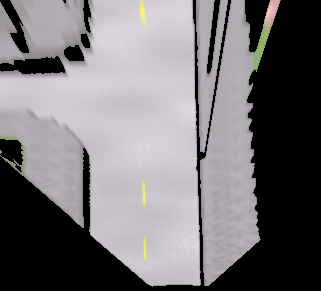
\includegraphics[width=.6\linewidth]{img/filtromalo.png}
    \caption{Ejemplo de aislamiento incorrecto de las marcas en la calzada}
    \label{fig:filtroMalo}
\end{figure}


\begin{figure}[h!]
    \centering
    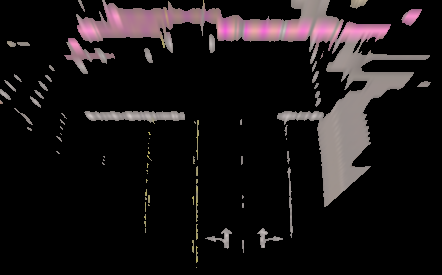
\includegraphics[width=.8\linewidth]{img/frontMasked.png}
    \caption{Vista cenital de la zona delante del vehículo con filtro de marcas en calzada aplicado.}
    \label{fig:frontMasked}
\end{figure}




\clearpage
\paragraph{\textit{Template Matching} con OpenCV}\mbox{}\\
Para la identificación de las marcas en la calzada utilizamos un sistema de detección mucho más simple.
Puesto que las marcas como pasos de peatones, flechas de dirección y letras de STOP se adhieren a un standard y siempre son iguales se ha investigado la identificación de estas mediante la técnica de \textit{Template Matching}.

Para ello, se utilizan los patrones que se pueden comprobar en la figura \ref{fig:templatespatter}. El algoritmo de OpenCV se encarga de devolvernos, en el caso de que detecte algún patrón, la posición de la imagen en la que se está detectando.

En el fragmento de código \ref{cod:mathctemplate} se pueden observar las llamadas a los distintos detectores y en la figura \ref{fig:inmeditamenteDelante} podemos ver un ejemplo de detección correcta.

\begin{figure}[h!]
    \centering
    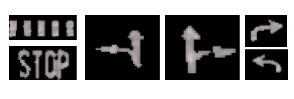
\includegraphics[width=.8\linewidth]{img/TemplatesPatternMatching.png}
    \caption{\textit{Templates} utilizadas para el reconocimiento mediante patrones de OpenCV}
    \label{fig:templatespatter}
\end{figure}

\begin{figure}[h!]
    \centering
    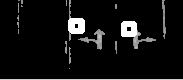
\includegraphics[width=.8\linewidth]{img/inmeditamenteDelante.png}
    \caption[Detección de marcas en la calzada con \textit{template matching}]{Recorte de la vista cenital. Los cuadrados indican la correcta identificación de la marca en la calzada}
    \label{fig:inmeditamenteDelante}
\end{figure}

\begin{lstlisting}[h!, language=python,caption=Fragmento de código utilizado para la deteccion de marcas en calzada, label={cod:mathctemplate}]
img = cv2.cvtColor(img, cv2.COLOR_BGR2GRAY)
    
matchsSTOP = cv2.matchTemplate(img, self.templateSTOP, cv2.TM_CCOEFF_NORMED)
matchsCebra = cv2.matchTemplate(img, self.templateCebra, cv2.TM_CCOEFF_NORMED)

matchsDelanteDerecha = cv2.matchTemplate(img, self.templateDelanteDerecha, cv2.TM_CCOEFF_NORMED)
matchsDelanteIzq= cv2.matchTemplate(img, self.templateDelanteIzq, cv2.TM_CCOEFF_NORMED)

matchsIzq = cv2.matchTemplate(img, self.templateIzq, cv2.TM_CCOEFF_NORMED)
matchsDerecha = cv2.matchTemplate(img, self.templateDerecha, cv2.TM_CCOEFF_NORMED)
\end{lstlisting}




\clearpage
\subsection{Analizando los datos}

\subsubsection{Clasificación del estado de los semáforos} \label{sec:clasificacionSemáforos}

La selección del semáforo principal, es decir, la selección del semáforo que se encuentra afectando a nuestro vehículo, es sin duda un problema con una dificultad mucho mayor que la de su detección \cite{karpathyAI}. 
Por esto, nuestra \textit{approach} a este problema se ha basado en realizar una selección muy sencilla.
En nuestro caso, consideraremos como  semáforo principal aquel que se encuentre más cerca del punto central de la horizontal de la imagen de la cámara principal tal y como se puede comprobar en la figura \ref{fig:semaforoPrincipal}.
Este comportamiento simplifica considerablemente la decisión de selección del semáforo que afecta al vehículo y nos ofrece unos resultados relativamente buenos puesto que, generalmente, el semáforo que afecta a nuestro vehículo se encontrará frente a este.

\begin{figure}[h!]
    \centering
    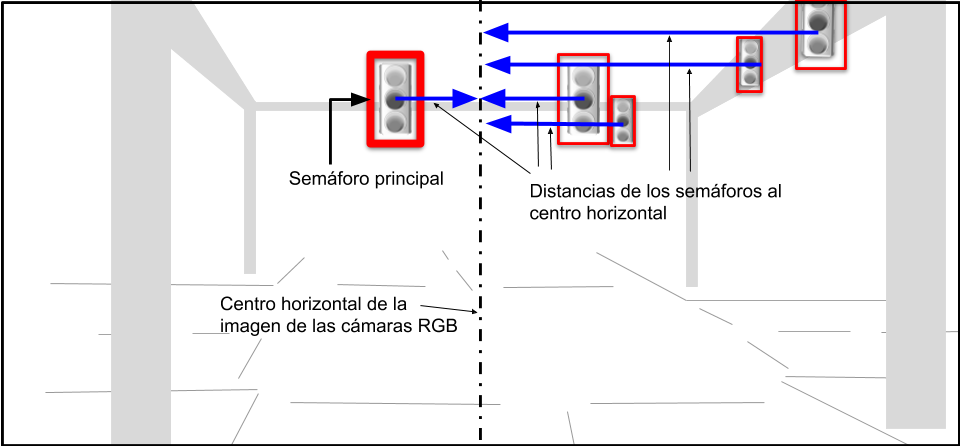
\includegraphics[width=\linewidth]{img/semaforoPrincipal.png}
    \caption{Método de selección de semáforo principal}
    \label{fig:semaforoPrincipal}
\end{figure}

Una vez hemos seleccionado el semáforo que deberemos considerar necesitaremos realizar un recorte de la imagen para quedarnos con la región en la que se ha detectado el semáforo.
Sin embargo, debido a que la calidad de las detecciones del módulo de detección de objetos dejan bastante que desear también tenemos en cuenta un pequeño \textit{padding} que nos permitirá asegurarnos de que el semáforo se encontrará dentro del rectángulo que recortaremos.

Una vez hayamos realizado el recorte procederemos a cambiar el tamaño de la imagen a una imagen de 25x25 pixeles, que es el tamaño que espera el modelo de clasificación.
\begin{figure}[h!]
    \centering
    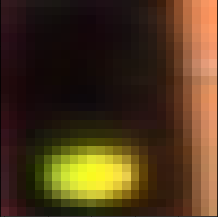
\includegraphics[width=.25\linewidth]{img/semaf25x25.png}
    \caption{Recorte y ajuste del tamaño del semáforo a una imagen de 25x25 píxeles}
    \label{fig:semaf25x25}
\end{figure}




\paragraph{Modelo de clasificación de semáforos}\mbox{}\\

Para la detección del estado del semáforo se ha utilizado un clasificador binario entrenado sobre el dataset LISA.

La estructura de la red se compone de una simple capa de Conv2D, su correspondiente MaxPooling, dos capas de 10 neuronas \textit{fully-connected} y como salida de la red una única neurona cuya salida se corresponde con la función de activación sigmoide.

\begin{figure}[h!]
    \centering
    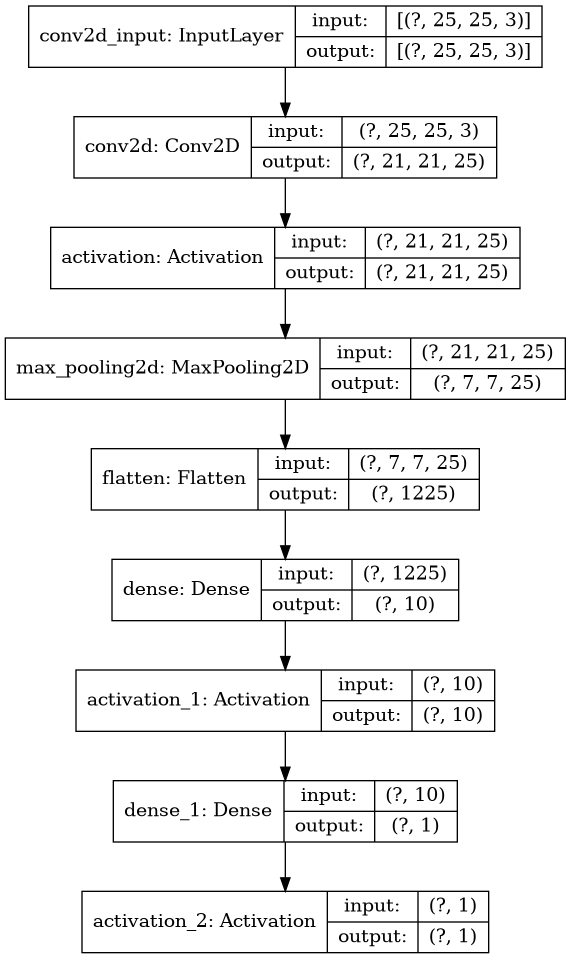
\includegraphics[width=0.6\linewidth]{img/DiagramaModeloSemaf.png}
    \caption{Estructura del modelo de detección del estado del semáforo}
    \label{fig:diamSemaf}
\end{figure}

Una vez realizado el entrenamiento se obtuvieron los resultados que se pueden comprobar en la figura \ref{fig:graficasSemaf}, los cuales son realmente buenos. La gran exactitud de las predicciones de este modelo se puede atribuir al gran dataset que hemos utilizado para entrenarlo.

\begin{figure}[h!]
    \begin{subfigure}[c]{.5\textwidth}
      \centering
      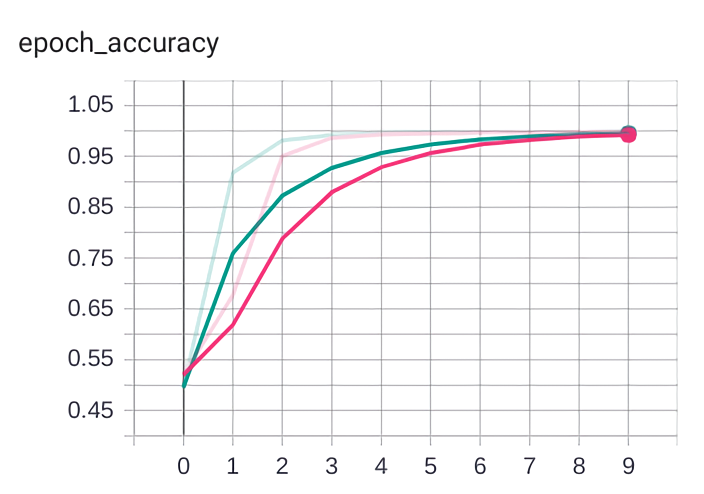
\includegraphics[width=.9\linewidth]{img/semafAcc.png}
      \caption[Precisión del entrenamiento del modelo de semáforos]{Evolución de la precisión durante el entrenamiento}
      \label{fig:semafacc}
    \end{subfigure}%
    \begin{subfigure}[c]{.5\textwidth}
      \centering
      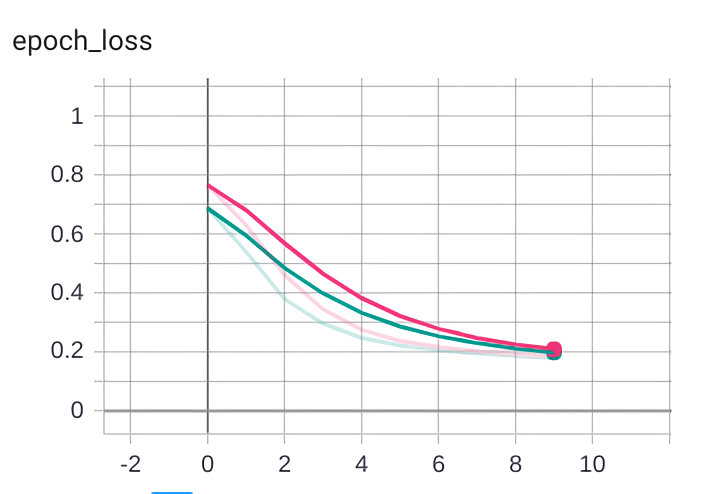
\includegraphics[width=.9\linewidth]{img/semafLoss.png}
      \caption[\textit{Loss} del entrenamiento del modelo de semáforos]{Evolución de la función \textit{loss} durante el entrenamiento}
      \label{fig:semafloss}
    \end{subfigure}
    
    \caption[Métricas obtenidas del entrenamiento del analizador de semáforos]{Métricas obtenidas durante el entrenamiento de la red convolucional. Las líneas azul y rosa indican la precisión y \textit{loss} sobre el conjunto de entrenamiento y validación respectivamente.}
    \label{fig:graficasSemaf}
\end{figure}

A pesar de estos resultados siempre es posible que la red realice predicciones erróneas por lo que siempre devolvemos el valor más repetido de las últimas 10 predicciones.



\subsubsection{Algoritmo de seguimiento de vehículos y predicción de la posición futura} \label{sec:algoritmoSeguimiento}

A pesar de haber realizado la detección de objetos con el módulo de detección de objetos, aún debemos tratar estos datos para intentar obtener algún conocimiento sobre estos. Para ello utilizaremos el algoritmo de seguimiento de vehículos que se explica a continuación.

El algoritmo utilizado para el seguimiento de vehículos es un algoritmo de invención propia que intenta relacionar las detecciones del frame actual con las del frame anterior y asignarle el mismo identificador. 
Gracias a este algoritmo podremos identificar si un vehículo detectado es el mismo que uno que ya había sido detectado anteriormente y realizar un seguimiento de su posición que nos permita obtener aún más información.

Esta relación de las detecciones con las del frame anterior se realiza teniendo en cuenta las distancias de los puntos centrales de las detecciones (tanto del frame actual como del anterior), de forma que la detección de un vehículo será relacionada con la detección del fotograma anterior (es decir consideraremos dos detecciones como un único vehículo que se ha movido y no como dos vehículos distintos) siempre y cuando la distancia entre las detecciones del frame $t-1$ y $t$ se encuentren lo suficientemente cerca.

En nuestro sistema se ha elegido un valor de distancia entre dos detecciones de 300 píxeles. Este valor ha sido definido mediante la experimentación.

En la figura \ref{fig:trackingVehiculos} se puede observar un pequeño diagrama que ayudará a la comprensión del funcionamiento de este algoritmo.

\begin{figure}[h!]
    \centering
    \includegraphics[width=\linewidth]{img/Algoritmo de tracking vehículos.png}
    \caption[Diagrama de funcionamiento del algoritmo de seguimiento de vehículos]{Diagrama de funcionamiento del algoritmo de seguimiento de vehículos. En este caso el vehículo de la izquierda será relacionado con el vehículo con identificador ``X''. En el caso del vehículo de la derecha este será relacionado con el vehículo con ID ``Y'' puesto que esa antigua predicción es la más cercana.}
    \label{fig:trackingVehiculos}    
\end{figure}


A medida que vamos relacionando los vehículos con las predicciones anteriores podemos ir guardando las posiciones de estos para de esta forma tener una `memoria' de posiciones que nos permitirá intentar predecir la posición futura de este.

La predicción futura de la posición del vehículo se realiza con la ayuda de la función polyfit de la librería numpy.

\begin{figure}[h!]
    \centering
    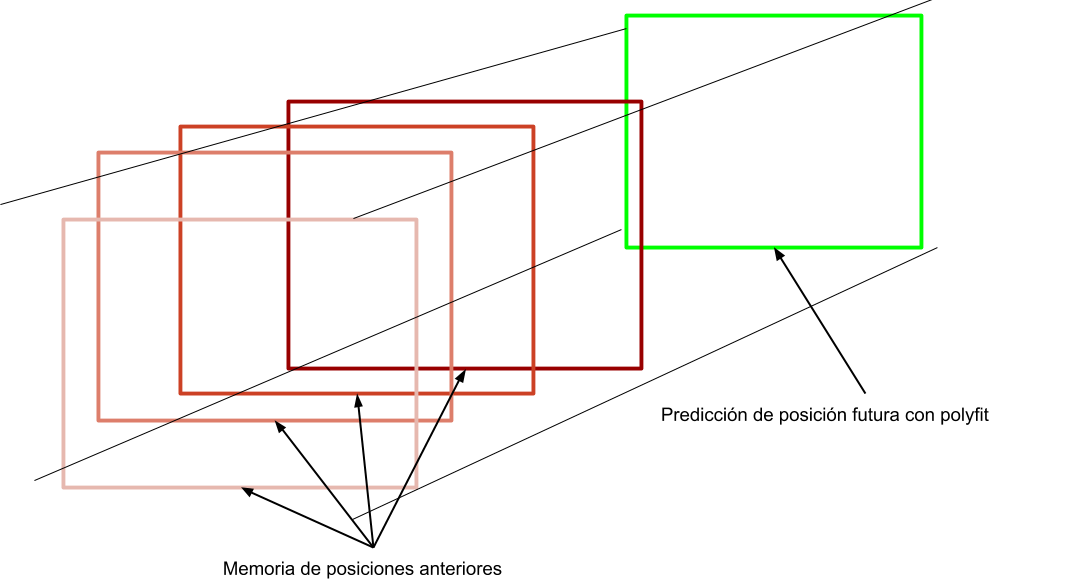
\includegraphics[width=\linewidth]{img/Posicionfutura.png}
    \caption{Predicción de posición futura del vehículo}
    \label{fig:posicionfutura}    
\end{figure}

Una vez tengamos la predicción de la posición futura del vehículo podremos calcular si nos estamos acercando o alejando de él. Este cálculo se realiza comparando el ancho de la detección actual y el ancho de la predicción. Si este ancho aumenta esto indicará que nos estamos acercando al vehículo, si por el contrario el ancho disminuye esto nos indicará que el vehículo se está alejando.


\clearpage
\subsubsection{Algoritmo de seguimiento de peatones}
El algoritmo de predicción de la posición de peatones es similar al de la predicción de posición de vehículos. La única diferencia importante es que las detecciones de entrada se corresponden con las de los peatones y no las de los vehículos.

Si la predicción de la posición futura del peatón está lo bastante cerca del punto medio horizontal de la imagen de las cámaras activaremos el indicador visual correspondiente con el paso de peatones.

\begin{figure}[h!]
    \centering
    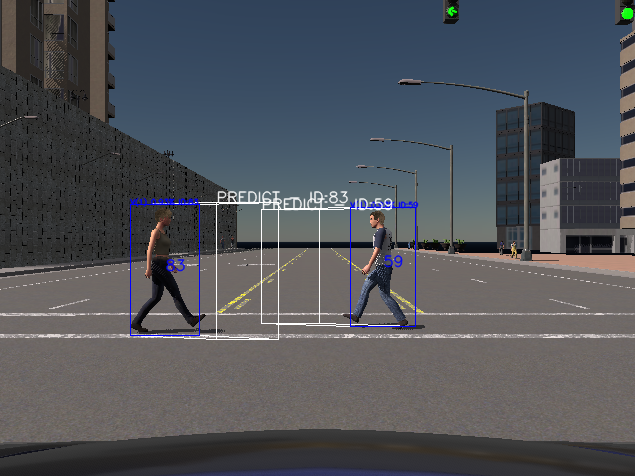
\includegraphics[width=0.9\linewidth]{img/peatones.png}
    \caption{Predicción de posición futura de peatones}
    \label{fig:peatones}    
\end{figure}


\clearpage
\subsection{Toma de decisiones}

A continuación se explica cómo se realiza la toma de deciciones que nos permite saber si se deben mostrar y reproducir notificaciones.

\subsubsection{Control del límite de velocidad}
El control del límite de velocidad es sin duda una de las decisiones más simples que nuestro sistema realiza. 
Esta decisión se trata de la comparación entre la velocidad actual del vehículo y la velocidad del límite de velocidad detectado por el módulo de detección.
Si la velocidad actual del vehículo es mayor que la velocidad del límite de velocidad decidiremos actuar ante esta situación permitiendo que la interfaz gráfica y el módulo de notificaciones muestren y hagan sonar la notificación correspondiente.

\subsubsection{Control de la atención del conductor}
Para el control de la atención del conductor utilizamos la información obtenida desde el servidor de atención para iniciar un temporizador cuando el conductor deja de estar atento.
Una vez este temporizador haya alcanzado un valor de 1.5 segundos permitimos que la interfaz gráfica muestre la notificación visual y que el módulo de notificaciones auditivas comience a reproducir un sonido hasta que el conductor vuelva a estar atento.

\subsubsection{Aviso de cambio de semáforo}
En cuanto a la notificación de cambio de semáforo esta se emite cuando se detecta un cambio del semáforo principal, desde la información que nos proporciona el módulo de clasificación de semáforos, desde el color rojo al color verde. La notificación desaparecerá cuando las cámaras dejen de ver el semáforo principal o cuando este vuelva a cambiar al color rojo.
Un ejemplo de la notificación que se muestra se podrá encontrar en la figura \ref{fig:notificaciones}.

\subsubsection{Aviso de vehículo en ángulo muerto}
Otro tipo de análisis que realizamos es la identificación de vehículos en el ángulo muerto del vehículo. Para ello utilizamos los datos del detector de objetos y en el caso de que detectemos algún vehículo en la imagen de las cámaras que miran hacia atrás comprobamos su área para conocer si se encuentra cerca o no.
En el caso de que se encuentre lo suficientemente cerca como para que suponga un problema se activa el indicador de vehículo en ángulo muerto tal y como se puede ver en la figura \ref{fig:angulomuerto}.

\begin{figure}[h!]
    \centering
    \includegraphics[width=\linewidth]{img/angulomuerto.png}
    \caption{Indicación de vehículo en ángulo muerto}
    \label{fig:angulomuerto}    
\end{figure}


\subsubsection{\textit{Road director}} \label{sec:roadDire}
El modulo \textit{Road director} es el encargado de llevar un seguimiento de la posición del volante del conductor y compararlo con la posición predecida por una red entrenada con información del sistema \textit{autopilot} del simulador.

De esta forma, si existe una gran diferencia entre la posición del volante del conductor y la posición que el sistema espera se activarán las notificaciones correspondientes.

El nombre \textit{Road director} viene inspìrado por el sistema \textit{Flight director} de los sistemas \textit{autopilot} de la aeronaves, cuya función es la de indicarle al piloto la maniobra que el sistema realizaría si este se encontrase en control del avión.

\begin{figure}[h]
    \centering
    \includegraphics[width=0.5\linewidth]{img/FlightDirector.png}
    \caption[El director de vuelo (\textit{Flight director}) en la pantalla principal de vuelo de una aeronave]{Director de vuelo (\textit{Flight director}) en la pantalla principal de vuelo de una aeronave. La cruz de color rosa indica la maniobra que el \textit{autopilot} del avión realizaría si tuviese el control. En este caso el avión se encuentra nivelado por lo que se mantendría el rumbo sin modificación alguna.}
    \label{fig:flightDirector}
\end{figure}
\begin{figure}[h!]
    \centering
    \includegraphics[width=0.8\linewidth]{img/rdwheel.png}
    \caption{Visualización del ángulo de volante real y predecido}
    \label{fig:rdwheel}    
\end{figure}


Para conseguir realizar la comparación entre estos dos valores será necesario obtener el valor que el sistema espera del conductor, para esto se ha utilizado una red neuronal que observando la imagen cenital de la zona inmediatamente delante del vehículo es capaz de devolvernos un valor que podemos transformar al rango comprendido entre el valor -0.7 y 0.7, que tal y como se ha visto en la sección \ref{sec:datossensores} se trata del mismo rango que los datos que obtenemos del sensor de ángulo de volante.

\paragraph{Entrenamiento y resultados obtenidos}\mbox{}\\
Esta red neuronal ha sido entrenada con el dataset explicado en la sección \ref{sec:datasetRD}.
Hasta el momento los resultados obtenidos no son satisfactorios y por lo tanto no se está realizando ninguna toma de decisiones que permita realizar notificaciones acústicas o visuales. El hecho de que no sean completamente satisfactorios no indica que no se encuentre funcionando correctamente, de hecho bajo ciertas circunstancias el funcionamiento es el correcto sin embargo, como no es completamente correcto finalmente se decidió deshabilitar la capacidad de enviar notificaciones.







\clearpage
\subsection{Interfaz gráfica y notificaciones visuales}

Una de las formas más efectivas de que el usuario se encuentre cómodo al utilizar nuestro sistema es asegurarnos de presentar la información que estamos obteniendo y analizando de una forma simple que permita al usuario comprobar que todo está funcionando correctamente.
Para cumplir con este cometido, y por supuesto cumplir uno de los objetivos indicados en la sección \ref{sec:Objetivos}, desde el comienzo del proyecto siempre se ha tenido en cuenta la necesidad de representar los datos en pantalla.

\subsubsection{Interfaz inicial basada en OpenCV}
Las primeras versiones de esta aplicación utilizaban como interfaz gráfica una única imagen generada con la librería OpenCV, en la que se iba superponiendo distinta información.

\begin{figure}[h!]
    \begin{subfigure}[c]{.5\textwidth}
      \centering
      \includegraphics[width=.9\linewidth]{img/InterfazCV2_1.png}
      \caption{Salida del detector de objetos}
      \label{fig:interfaz_cv_1}
    \end{subfigure}%
    \begin{subfigure}[c]{.5\textwidth}
      \centering
      \includegraphics[width=.9\linewidth]{img/InterfazCV2_2.png}
      \caption{Salida del detector de semáforos}
      \label{fig:interfaz_cv_2}
    \end{subfigure}
    
    \caption[Ejemplos de interfaz gráfica generada con OpenCV]{Ejemplos de interfaz gráfica generada con OpenCV. En las dos imágenes anteriores se pueden observar las distintas salidas sobrepuestas sobre las imágenes de las cámaras}
    \label{fig:interfaz_cv}
\end{figure}




\subsubsection{Interfaz gráfica con Qt5}

Más tarde, durante el desarrollo de la aplicación se decidió cambiar a una interfaz gráfica desarrollada con Qt que nos permitiera tener opciones más interesantes que las que podríamos conseguir con modificaciones sobre una imagen en OpenCV. En la figura \ref{fig:interfaz} se puede observar una captura de esta interfaz durante el funcionamiento del sistema.

\begin{figure}[h!]
    \centering
    \includegraphics[width=0.95\linewidth]{img/interfazJetson.png}
    \caption{Captura de la interfaz gráfica desarrollada}
    \label{fig:interfaz}    
\end{figure}

\clearpage
\paragraph{Cámaras, detección de objetos y vista cenital}\mbox{}\\
Aunque finalmente se decidiese utilizar Qt para la elaboración de la interfaz gráfica no se dejó de utilizar OpenCV para generar \textit{overlays} en las imágenes de las cámaras.
En concreto, en la nueva interfaz gráfica se utiliza gran parte de las imágenes generadas con OpenCV como por ejemplo en la vista cenital y en las cámaras RGB con la información del detector de objetos.

\paragraph{Indicadores}\mbox{}\\

Los indicadores de la interfaz simulan el comportamiento de un panel de instrumentos clásico en el que estos se encienden a medida se van detectando las distintas situaciones. Un gran ejemplo de estos indicadores son el indicador de límite de velocidad, que indica el límite de velocidad obtenido desde el simulador y el indicador de semáforo, que indica el estado del semáforo que está afectando al vehículo si se detecta alguno.

\paragraph{Notificaciones}\mbox{}\\

A medida que se vayan produciendo situaciones que requieran de una notificación visual estas aparecerán en la zona de notificaciones. Algunas de las notificaciones que se han considerado pueden verse en la figura \ref{fig:notificaciones}.

\begin{figure}[h]
    \centering
    \includegraphics[width=0.8\linewidth]{img/Notificaciones.png}
    \caption{Notificaciones visuales consideradas en la interfaz}
    \label{fig:notificaciones}    
\end{figure}


\paragraph{\textit{Road Director}}\mbox{}\\
En la zona de \textit{Road Director} podemos ver una comparativa entre la posición real del volante y la posición que el sistema tomaría de acuerdo a lo descrito en la sección \ref{sec:roadDire}




\clearpage
\subsection{Notificaciones auditivas} 
\subsubsection{Reproducción de sonidos con playsound} \label{playsound}
Inicialmente la reproducción de sonidos se realizaba con el módulo \textit{playsound}, sin embargo, debido a varios problemas de compatibilidad con el entorno de desarrollo se decidió cambiar y utilizar un reproductor para reproducir las notificaciones auditivas.

\subsubsection{Reproducción de sonidos con mpv}
Finalmente, para evitar problemas en el sistema de desarrollo se eligió utilizar un reproductor de audio y video para reproducir las señales acústicas.
En concreto se está utilizando el reproductor \texttt{mpv} al cual se llama mediante una llamada a la función \texttt{sys.os} de python.

La clase completa que se encarga de reproducir las alertas de sonido es la que se puede observar en el fragmento de código \ref{cod:mpv}
\begin{lstlisting}[h!, language=python,caption=Clase encargada de la reproducción de notificaciones acústicas, label={cod:mpv}]
class notificacionesSonido:

    def __init__(self):
        
        self.sonido = None

        # Thread
        t = threading.Thread(target=self._reproduceSonidoSiHayCola)
        t.daemon = True
        t.start()
        
    def _reproduceSonidoSiHayCola(self):
        while True:
            if self.sonido is not None:
                print('Sonido!')
                os.system(f'mpv resources/quindarTones/{self.sonido}.ogg')
                self.sonido = None

            time.sleep(0.1)

    def reproduceAlertaQuindarStart(self):
        self.sonido = 'start'

    def reproduceAlertaQuindarEnd(self):
        self.sonido = 'end'
\end{lstlisting}


\clearpage
\section{Pruebas del sistema} \label{sec:pruebas}

Durante todo el desarrollo del proyecto se ha ido comprobando la correcta ejecución de todos los sistemas, pero para obtener unos resultados concretos hemos realizado distintas pruebas. A continuación, en la tabla \ref{tab:pruebas} ofrecemos los resultados de estas.

\begin{table}[h!]
    \centering
    \resizebox{\textwidth}{!}{%
    \begin{tabular}{@{}lllll@{}}
    \toprule
    \multicolumn{5}{c}{Resultados de las distintas pruebas realizadas}                                                              \\ \midrule
    Tipo de prueba                                  & Pruebas realizadas & Aciertos & Fallos & Porcentaje de aciertos               \\ \midrule
    Detección del límite de velocidad               & 20                 & 20       & 0      & 100\%      \footnotemark             \\
    Detección de marca de STOP en calzada           & 20                 & 18       & 2      & 90\%                                 \\
    Detección de semáforos                          & 50                 & 35       & 15     & 70\%                                 \\
    Correcta clasificación del estado del semáforo  & 50                 & 33       & 17     & 66\%                                 \\
    Notificación de cambio de semáforo              & 30                 & 28       & 2      & 93.3\%                               \\
    Reacción ante pérdida de atención del conductor & 20                 & 20       & 0      & 100\%                                \\
    Correcta predicción de intersección             & 50                 & 42       & 8      & 84\%                                 \\
    Correcta detección de marcas en la calzada     & 70                 & 59       & 11     & 84.29\%                              \\ \bottomrule
    \end{tabular}%
    }
    \caption{Resultados obtenidos durante las pruebas del sistema}
    \label{tab:pruebas}
\end{table}
\footnotetext{El porcentaje de acierto es un 100\% porque se están utilizando los datos que nos aporta el simulador}


A continuación se destacan los puntos más importantes acerca de los aciertos y fallos obtenidos en las pruebas.

\begin{itemize}
    \item \textbf{Detección de marca de STOP en calzada:} Cuando el vehículo se acerca a una marca de STOP desde un ángulo no natural el detector tiene problemas para detectar la marca.
    \item \textbf{Detección de semáforos:} El detector de objetos tiene problemas distinguiendo los semáforos que tienen algún edificio detrás. Algunas veces también detecta, erróneamente, semáforos en las copas de los árboles. Bajo ciertas circunstancias, el rectángulo de la predicción aparece en una posición un poco alejada y no contiene al semáforo.
    \item \textbf{Notificación de cambio de semáforo:} La notificación de cambio de semáforo no se lanza si se pierde la detección del semáforo en el momento en el que este cambia.
    \item  \textbf{Correcta clasificación del estado del semáforo:} Cuando la zona recortada no contiene un semáforo la mayoría de las veces se considera un semáforo en verde. Si el semáforo es muy pequeño también existen problemas al detectar el estado.
    \item \textbf{Correcta predicción de intersección:} Para algunos tipos de intersecciones extrañas el detector no es capaz de reconocerlas correctamente, algo razonable debido a la poca cantidad de imágenes del dataset que se ha utilizado.
    
\end{itemize}

Otro de los puntos interesantes a destacar es la velocidad de procesamiento que se obtiene al ejecutar el sistema en el dispositivo NVIDIA Jetson AGX Xavier. Con el perfil de consumo máximo de energía, el cual se corresponde con 30W, obtenemos aproximadamente unos 15 FPS con picos de 18 FPS un valor muy bueno puesto que nos mantenemos en un margen que se puede considerar \textit{real-time} y que, además, se asimila a la velocidad de procesamiento de otras soluciones con un mayor consumo de energía como por ejemplo el sistema Tesla \textit{autopilot} (en la figura \ref{fig:teslaautopilotvideorecruit}, obtenida de \cite{teslaautopilotrecruiting}, se puede observar como este sistema se mantiene entre 13 y 20 FPS. Este sistema está diseñado con una restricción de presupuesto de energía de 100W \cite{teslaAutonomyDay}).

	  \chapter{Planificación del proyecto}\label{capPlanificacion}
A continuación se realiza una explicacion extensiva de la planificación inicial y final de nuestro proyecto.





\section{Planificación temporal inicial}\label{sec:planTemporalInicial}

En la figura \ref{fig:ganttInicial} se puede observar el diagrama de Gantt con la planificación inicial de este proyecto.
\begin{figure}[h!]
    \centering
    \includegraphics[width=0.9\linewidth]{img/Inicial/gantt-inicial.png}
    \caption{Diagrama de Gantt de la planificación inicial}
    \label{fig:ganttInicial}    
\end{figure}

\section{Planificación financiera inicial}\label{sec:planFinancieroInicial}
En cuanto a la planificación financiera inicial, se esperaba que el desarrollo del proyecto costase aproximadamente unos 20.125\euro y que tuviese una evolución como la que se puede observar en la figura \ref{fig:gastosInicial}
\begin{figure}[h!]
    \centering
    \includegraphics[width=0.7\linewidth]{img/Inicial/costes.PNG}
    \caption{Diagrama de planificación de gastos inicial}
    \label{fig:gastosInicial}    
\end{figure}


\section{Retrasos provocados por diversos motivos y cambios en el trabajo}

A pesar de haber planificado la realización de las tareas del proyecto de acuerdo a lo descrito en los apartados anteriores, a medida que se iba realizando el proyecto se fueron encontrando diversas dificultades que impidieron el seguimiento de la planificación.

La primera de ellas fue el gran retraso que se produjo tras la imposibilidad de acceder al hardware de desarrollo debido al estado de alarma nacional decretado debido a la crisis sanitaria global provocada por el virus SARS-CoV-2.
Tras los retrasos provocados por la falta del hardware se decidió aplazar la fecha de entrega de este trabajo a la siguiente convocatoria. 

Durante el periodo de cuarentena también se decidió migrar la ejecución del sistema desde un vehículo real a un simulador ya que, debido a la situación, depender de la conducción de un vehículo real no parecía ser una opción razonable.

Finalmente otro de los problemas encontrados durante la elaboración del proyecto fue el cambio de dos a un único autor, lo que supuso una mayor carga de trabajo ya que, como se ha observado, incluso la planificación inicial del trabajo se trataba de una planificación para 2 personas.


\section{Planificación temporal final} \label{sec:planTemporalFinal}
Finalmente, tras los cambios, la planificación temporal al finalizar el trabajo coincide con la que se puede observar en la figura \ref{fig:ganttfinal}.
\begin{figure}[t]
    \centering
    \includegraphics[width=\linewidth]{img/Final/gantt.png}
    \caption{Diagrama de Gantt de la planificación final}
    \label{fig:ganttfinal}    
\end{figure}


\section{Planificación financiera final} \label{sec:planFinancieroFinal}
La planificación financiera final del trabajo se ha visto modificada para coincidir con la nueva planificación.
Tal y como se puede comprobar en la figura \ref{fig:gastosFinal} la cifra final asciende a 39.546 \euro. 
\begin{figure}[h!]
    \centering
    \includegraphics[width=0.7\linewidth]{img/Final/costes.PNG}
    \caption{Diagrama de planificación de gastos final}
    \label{fig:gastosFinal} 
\end{figure}



\section{Precios utilizados}
Los precios utilizados para el cálculo de la planificación financiera han sido un redondeo de los precios medios que se pueden observar en \cite{preciosInformatica}.
A modo informativo, en la tabla \ref{tab:precios} se pueden observar cuales han sido estas cantidades.

\begin{table}[h!]
    \centering
    \begin{tabular}{@{}ll@{}}
    \toprule
    Posición                                  & Salario/hora                         \\ \midrule
    Jefe de proyecto                          & 37 \euro                                 \\
    Analista                                  & 30 \euro                                  \\
    Desarrollador                             & 25 \euro                                  \\
    Diseñador                                 & 31 \euro                                  \\ \bottomrule
    \end{tabular}
    \caption{Precios utilizados para el cálculo de la planificación financiera}
    \label{tab:precios}
\end{table}




\section{Estudio de mercado} \label{sec:estudioDeMercado}
\subsection{Clientes potenciales} \label{sec:clientesPotenciales}

Los principales clientes potenciales de este sistema serán las empresas automovilísticas que no dispongan de un equipo centrado en el desarrollo de sistemas de conducción y que esten dispuestos a considerar una opción como la nuestra.

\subsection{Plan de comercialización} \label{sec:planComercializacion}

Teniendo en cuenta el precio final del sistema desarrollado y considerando lo que aportaría a una empresa automovilística, para la cual los precios de los extras suelen ser abismales creemos que el precio final al que se debería vender un sistema parecido al desarrollado sería de 50000 \euro, lo que nos proporcionaría un beneficio de 10454 \euro. Por otra parte, para la empresa el precio de este sistema sería bastante competitivo. Si Suponemos que un acuerdo con NVIDIA le permitiría obtener el hardware a un precio reducido de 500 \euro podrían recuperar la inversión en apenas la venta de 100 vehículos si se vende nuestro software en un paquete de 1000 \euro.

	  \chapter{Trabajo futuro}\label{capTrabajoFuturo}

\section{Aspectos a mejorar del proyecto}
Tal y como se ha comentado en el capítulo anterior existen bastantes puntos que podrían haber sido mejorados durante la elaboración de este proyecto.
De entre todos ellos a continuación realizaremos un pequeño comentario sobre los más interesantes.

\begin{itemize}
    \item Detección de señales de tráfico\\
        La detección del límite de velocidad finalmente se ha realizado obteniendo los datos de \textit{ground truth} desde el propio simulador. Uno de los aspectos que se debería considerar para ampliar en el futuro sería la detección de las señales de tráfico para permitir el funcionamiento de este sistema fuera de un simulador.

    \item Mejora del algoritmo de seguimiento de vehículos\\
        El algoritmo de seguimiento de vehículos explicado en la sección \ref{sec:algoritmoSeguimiento} podría ser modificado para mejorar el rendimiento así como la selección del vehículo del frame anterior con la que la nueva detección se corresponde.
        Para mejorar este algoritmo sería interesante relacionar las nuevas detecciónes con aquellas cuya intersección del area del rectángulo detectado y el área de los rectángulos de las detecciones anteriores sea máximo.

    \item Mejora de la selección del semáforo que afecta al vehículo\\
        Como se comentó en la sección \ref{sec:clasificacionSemáforos} la selección del semáforo principal se basa en la distancia de todos los semáforos detectados al centro de la imagen.
        Este sería uno de los aspectos a considerar más interesantes pero al mismo tiempo sería bastante complicado puesto que para obtener este conocimiento necesitaríamos obtener información mucho más precisa del espacio alrededor del vehículo.

    \item Obtención de otros tipos de datos del exterior del vehículo\\
        Un punto interesante que se consideró al comienzo del desarrollo y que lamentablemente se tuvo que omitir tras el cambio a trabajar con un simulador fue el uso de los micrófonos de las cámaras PS Eye para reconocer distintos tipos de señales acústicas.
        En un supuesto trabajo futuro de este proyecto este sería un punto bastante interesante, en especial si se combina con la posibilidad de testear nuestro sistema en un vehículo real.
\end{itemize}


\section{Testeo en un vehículo real}
Al comienzo del trabajo, antes de la decisión de cambiar a un simulador, se pensaba aplicar nuestro software a un vehículo real y permitir reaccionar ante las situaciones anómalas que se pudiera dar durante la conducción en entornos controlados.
Por supuesto, tras la decisión de realizar el proyecto con un simulador desechamos esta idea.
Una vez el sistema se haya mejorado sería interesante ejecutar este en un vehículo real y analizar los resultados que se obtienen.

\section{Independencia del hardware utilizado} \label{sec:independenciaHardware}
Otro de los puntos importantes a considerar en cuanto a trabajo futuro es la independencia del sistema con el hardware.
En el estado actual, tal y como se ha comentado en la sección \ref{sec:jetsonInference}, el detector de objetos se ha implementado utilizando una librería de NVIDIA.
En el mercado existen diversas opciones que se podrían considerar para sustituir a la librería \textit{jetson-inference} siendo la más interesante la propia API de detección de objetos de Tensorflow la cual ha sido recientemente actualizada para hacerla compatible con Tensorflow 2.0 que, como se ha comentado anteriormente, es la versión de Tensorflow que este proyecto está utilizando.

La reescritura del módulo de detección de objetos con una librería sin dependencias de hardware nos permitiría trasladar la ejecución de nuestro sistema a otros dispositivos empotrados así como en equipos de escritorio y, con gran seguridad, se obtendrían mejores resultados.


\section{Ejecución con un sistema mucho más potente}
De reescribirse el módulo de detección de objetos tal y como se ha comentado en la sección \ref{sec:independenciaHardware} el siguiente paso sería la ejecución del sistema en un equipo mucho más potente para de esta forma poder comprobar si los resultados obtenidos son mejores que los que se han especificado en \ref{sec:pruebas}.


	  \chapter{Conclusiones}
Debido al estado actual de elaboración del trabajo de Fin de Grado, el cual no ha avanzado mucho, aún no es posible sacar conclusiones sobre la realización y resultados de este.

Así pues esta sección no es más que un pequeño comentario para que la sección de apéndices no parezca encontrarse fuera de lugar.

	 


%     \input{Capitulos/capitulo2}
%     \input{Capitulos/defobjetivos}
%     \input{Capitulos/requisitos}
%     \input{Capitulos/analanteced}
%     \input{Capitulos/analtemporal}
%     \input{Capitulos/alternativas}
%     \input{Capitulos/pruebas}
%     \input{Capitulos/manual}


	%\bibliographystyle{sousa5}
	%\bibliographystyle{apacite}
	%\bibliographystyle{apalike}
	
	\bibliographystyle{IEEEtran}
	
	%\nocite{*} %Muestra toda la bibliografía, eliminar!!
	\renewcommand\bibname{Referencias bibliográficas}
	\bibliography{Bibliografia/bibliografia.bib}


\backmatter

	\chapter{Apéndices}\label{apendices}

%\section{Acta de adjudicación de TFG}
En la siguientes páginas se encuentran los distintos apéndices de este trabajo, entre los que se incluyen el acta de adjudicación asi como cualquier otro documento o información adicional que se haya referenciado anteriormente y se crea necesario.

\includepdf[pages=1,scale=.75,pagecommand=\section*{Acta de adjudicación}\label{apendice:actaadjudicacion}]{apendices/adjudicacion.pdf}

\end{document}
